% -*- root: ../main.tex -*-

% In questa sezione esporre brevemente i requisiti a cui il sistema proposto deve rispondere, concentrando l'attenzione sugli aspetti più rilevanti e facendo eventualmente uso di opportuni diagrammi di alto livello.
% 8000 - 10000 battute
% Attenzione in particolare ai requirement non funzionali: 1) non siano troppo vaghi altrimenti sono inverificabili, e quindi praticamente inutili; 2) se il sistema è distribuito, è inevitable dire cosa vi aspettate in termini di di robustezza a cambiamenti/guasti (quali?, come?), e scalabilità (in quale dimensione? fino a che punto?).

\chapter{Analisi dei Requisiti}
A seguito dell'intervista con l'esperto del dominio, sono emersi i seguenti requisiti per l'applicativo richiesto. Questi sono stati poi discussi e approvati dal committente.
\section{Requisiti di Business}
    L'importanza strategica del software risiede nel fornire agli studenti un valido strumento di ripasso e test delle competenze acquisite.
    Le aree semantiche di maggiore importanza sono l'interrogazione delle conoscenze tramite quesiti, il feedback sugli errori, la personalizzazione dei quiz, e delle statistiche globali e a fine partita. 
    I principali punti sono sotto riportati:
    \begin{itemize}
        \item selezione di N domande tra i C corsi scelti dell'utente
        \item gestione delle domande e delle relative risposte permettendo l'editing, il salvataggio e il caricamento delle stesse
        \item elaborare un riepilogo al termine di ogni partita
        \item elaborare e salvare alcune statistiche di interesse relativamente ad un utente
    \end{itemize}
	
\section{Requisiti Utente}
    Uno user dell'applicazione dovrà quindi essere in grado di:
    \begin{itemize}
        \item ripassare: visualizzare domande e scegliere tra le possibili risposte
        \item scegliere tra varie modalità di gioco
        \item visualizzare un riepilogo a fine partita
        \item visualizzare le proprie statistiche su tutte le partite effettuate
        \item importare ed esportare nuove domande e risposte indicando la materia a cui si riferiscono
    \end{itemize}
 
        \subsection{User Stories}
        \label{chap:UserStories}
        Si riportano di seguito le user stories emerse:
        \begin{itemize}
            \item Come utente voglio poter accedere all'applicativo e far iniziare una nuova partita;
            \item Come utente voglio poter selezionare la risposta che ritengo corretta, ricevendo un feedback a riguardo;
            \item Come utente voglio poter visualizzare le statistiche personali;
            \item Come utente voglio poter selezionare i corsi prima dell'inizio di ogni partita;
            \item Come utente voglio poter selezionare la modalità di gioco;
            \item Come utente voglio poter cambiare le impostazioni di gioco;
            \item Come utente voglio poter aggiungere domande, qualora volessi integrare nuovi quiz;
            \item Come utente voglio poter modificare domande aggiunte, qualora non siano corrette;
            \item Come utente voglio poter importare le domande in blocco relative a uno o più esami;
            \item Come utente voglio poter esportare le domande in blocco relative a uno o più esami;
            \item Come utente voglio poter riguardare i quiz della partita appena terminata.
        \end{itemize}
        
        \begin{figure}[H]
            \centering
            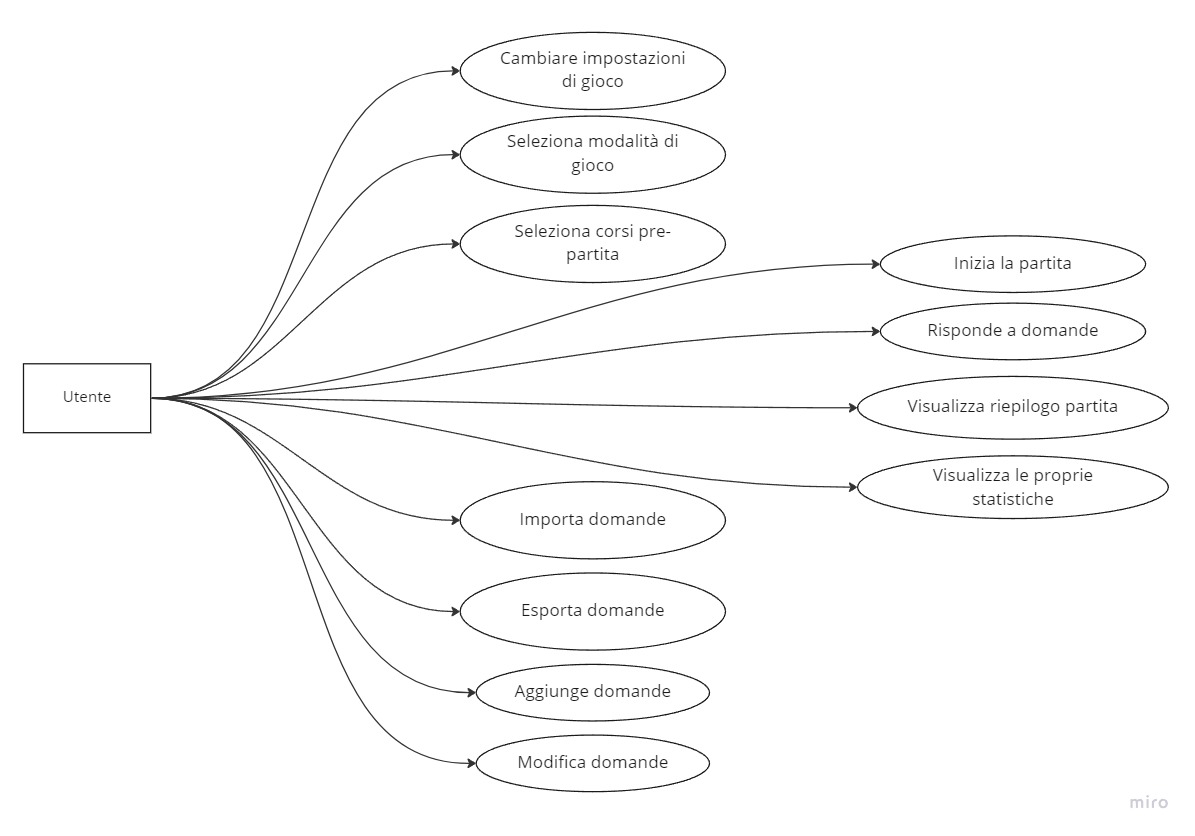
\includegraphics[width=\textwidth]{Miro/use-case.jpg}
            \caption{Schema Casi d'Uso}
            \label{fig:use-case}
        \end{figure}

        \subsection{Mockup}
        \label{chap:Mockup}
    	A seguito dell'intervista fatta con l'esperto del dominio e dei requisiti raccolti con esso, il team di sviluppo ha prodotto due versioni di mockup (\ref{mockup1} e \ref{mockup2}). In seguito, questi sono stati sottoposti al committente, il quale ha riscontrato aspetti positivi e negativi in entrambe le proposte. Di conseguenza, i mockup definitivi \ref{mockupFinished} sono stati sviluppati con la sua collaborazione e supervisione. Per garantire una maggior comprensione della navigazione all'interno dell'applicativo, è stato prodotto lo schema \ref{fig:mockup_nav}.
     
        \subsubsection{Mockup prima versione}\label{mockup1}
        
        \begin{figure}[H]
          \centering
          \begin{minipage}[b]{0.48\textwidth}
            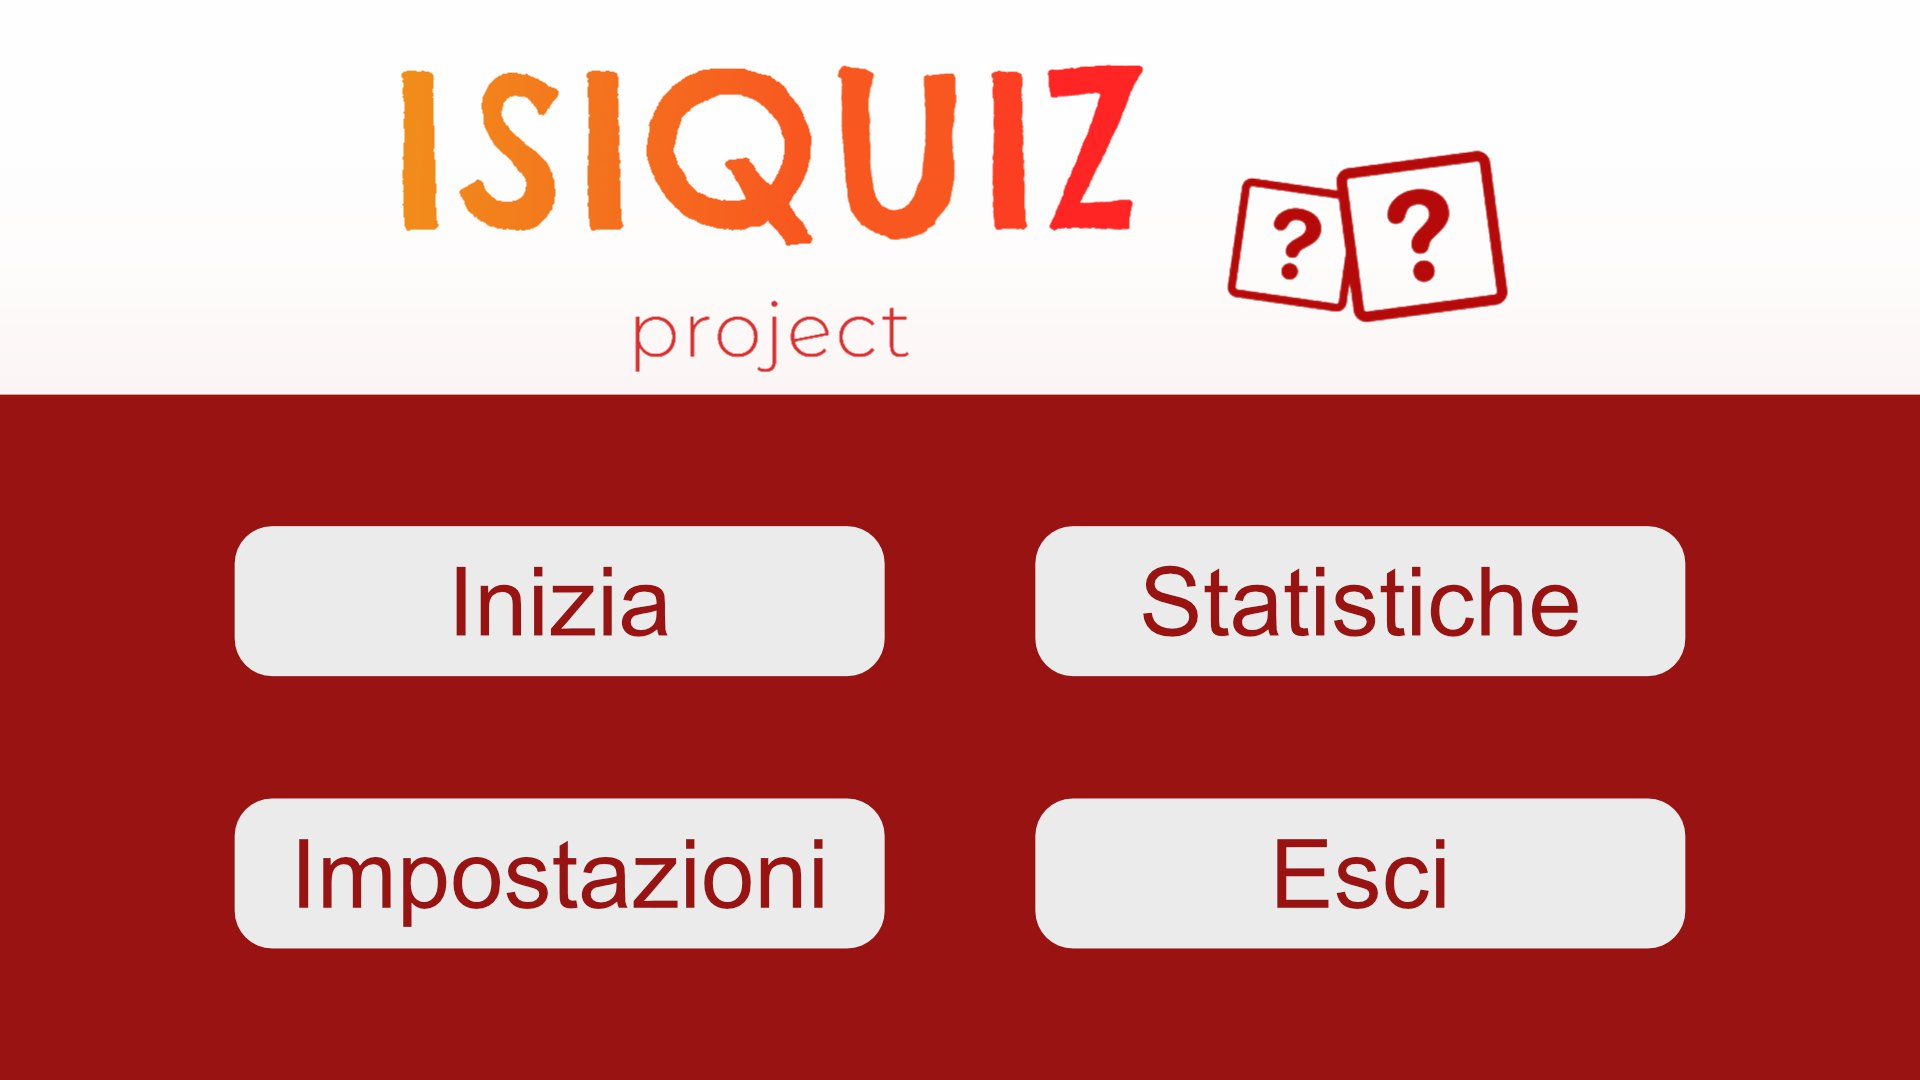
\includegraphics[width=\textwidth]{Images/mockup/home1.jpg}
            \caption{Pagina Iniziale}
            \label{fig:HomePage1}
          \end{minipage}
          \hfill
          \begin{minipage}[b]{0.48\textwidth}
            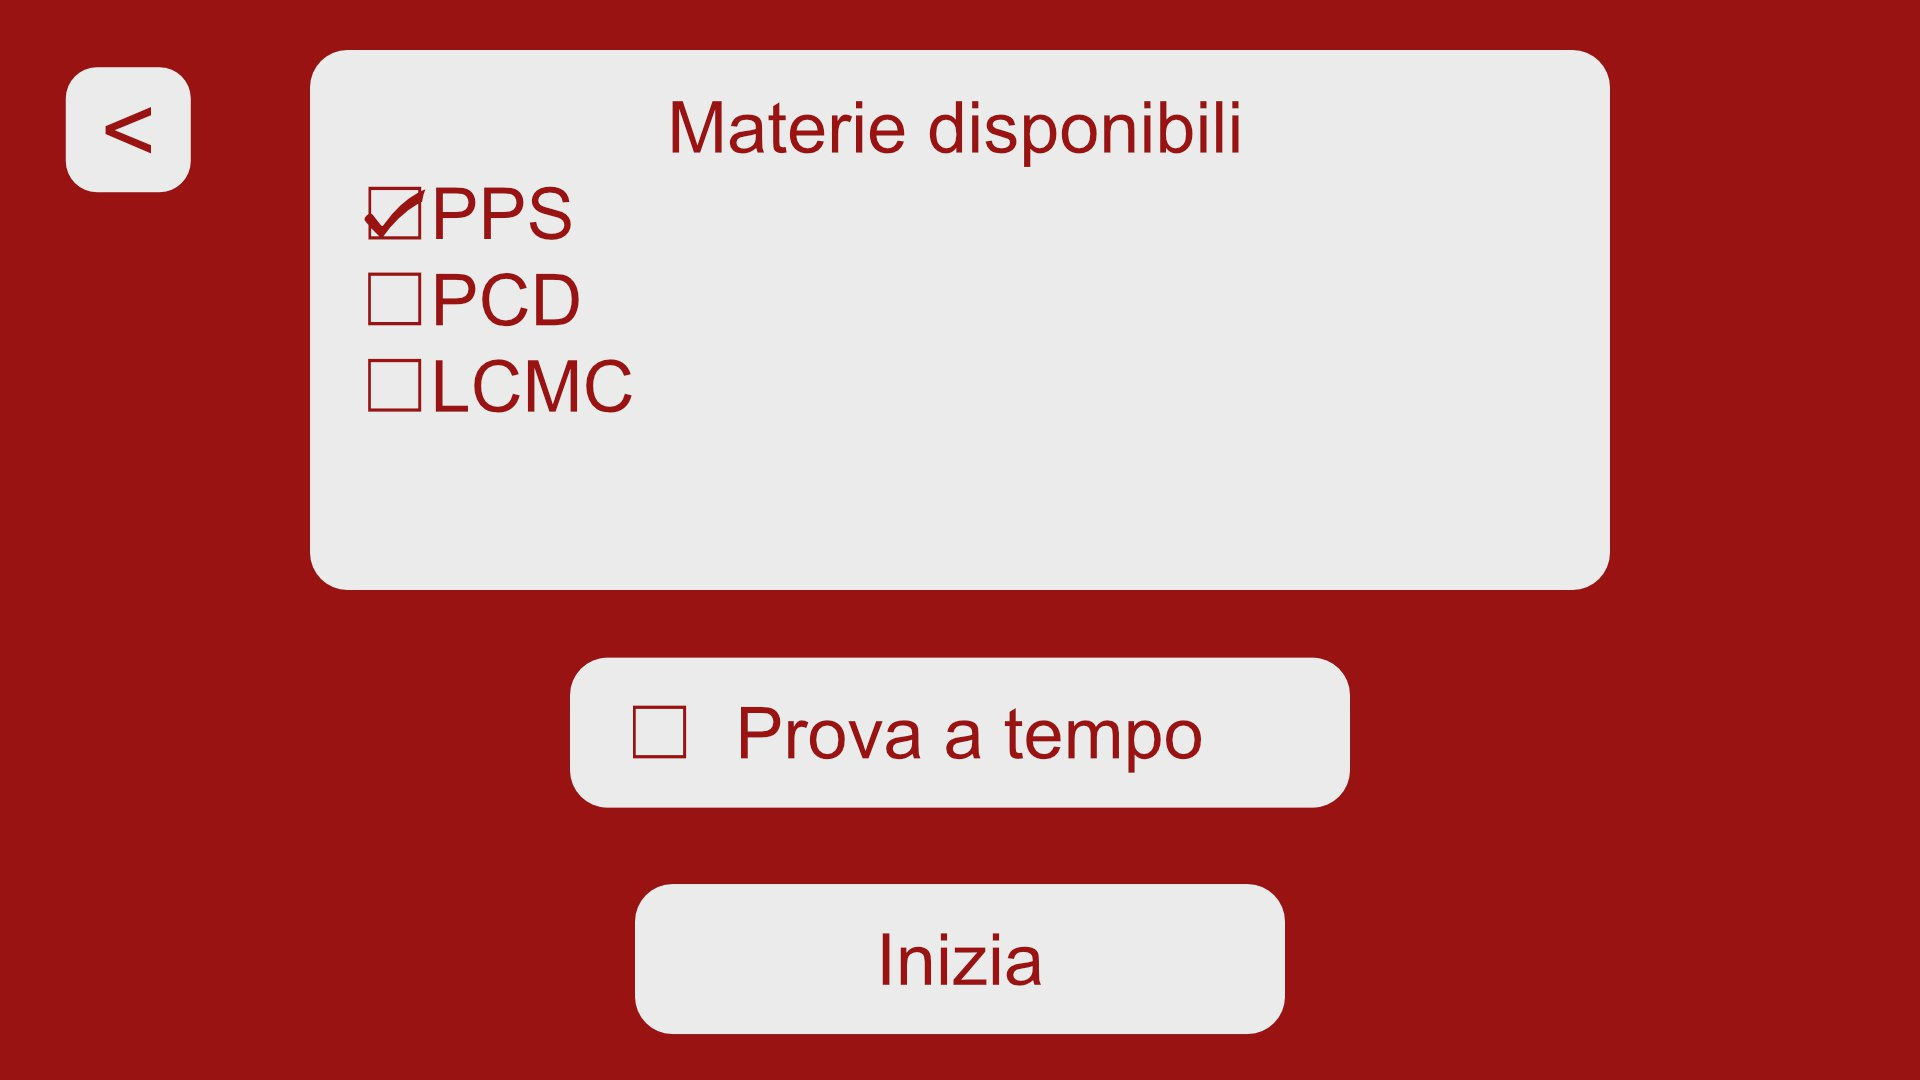
\includegraphics[width=\textwidth]{Images/mockup/start1.jpg}
            \caption{Settaggio di una partita prima di iniziarla}
            \label{fig:Start1}
          \end{minipage}
        \end{figure}

        \begin{figure}[H]
          \centering
          \begin{minipage}[b]{0.48\textwidth}
            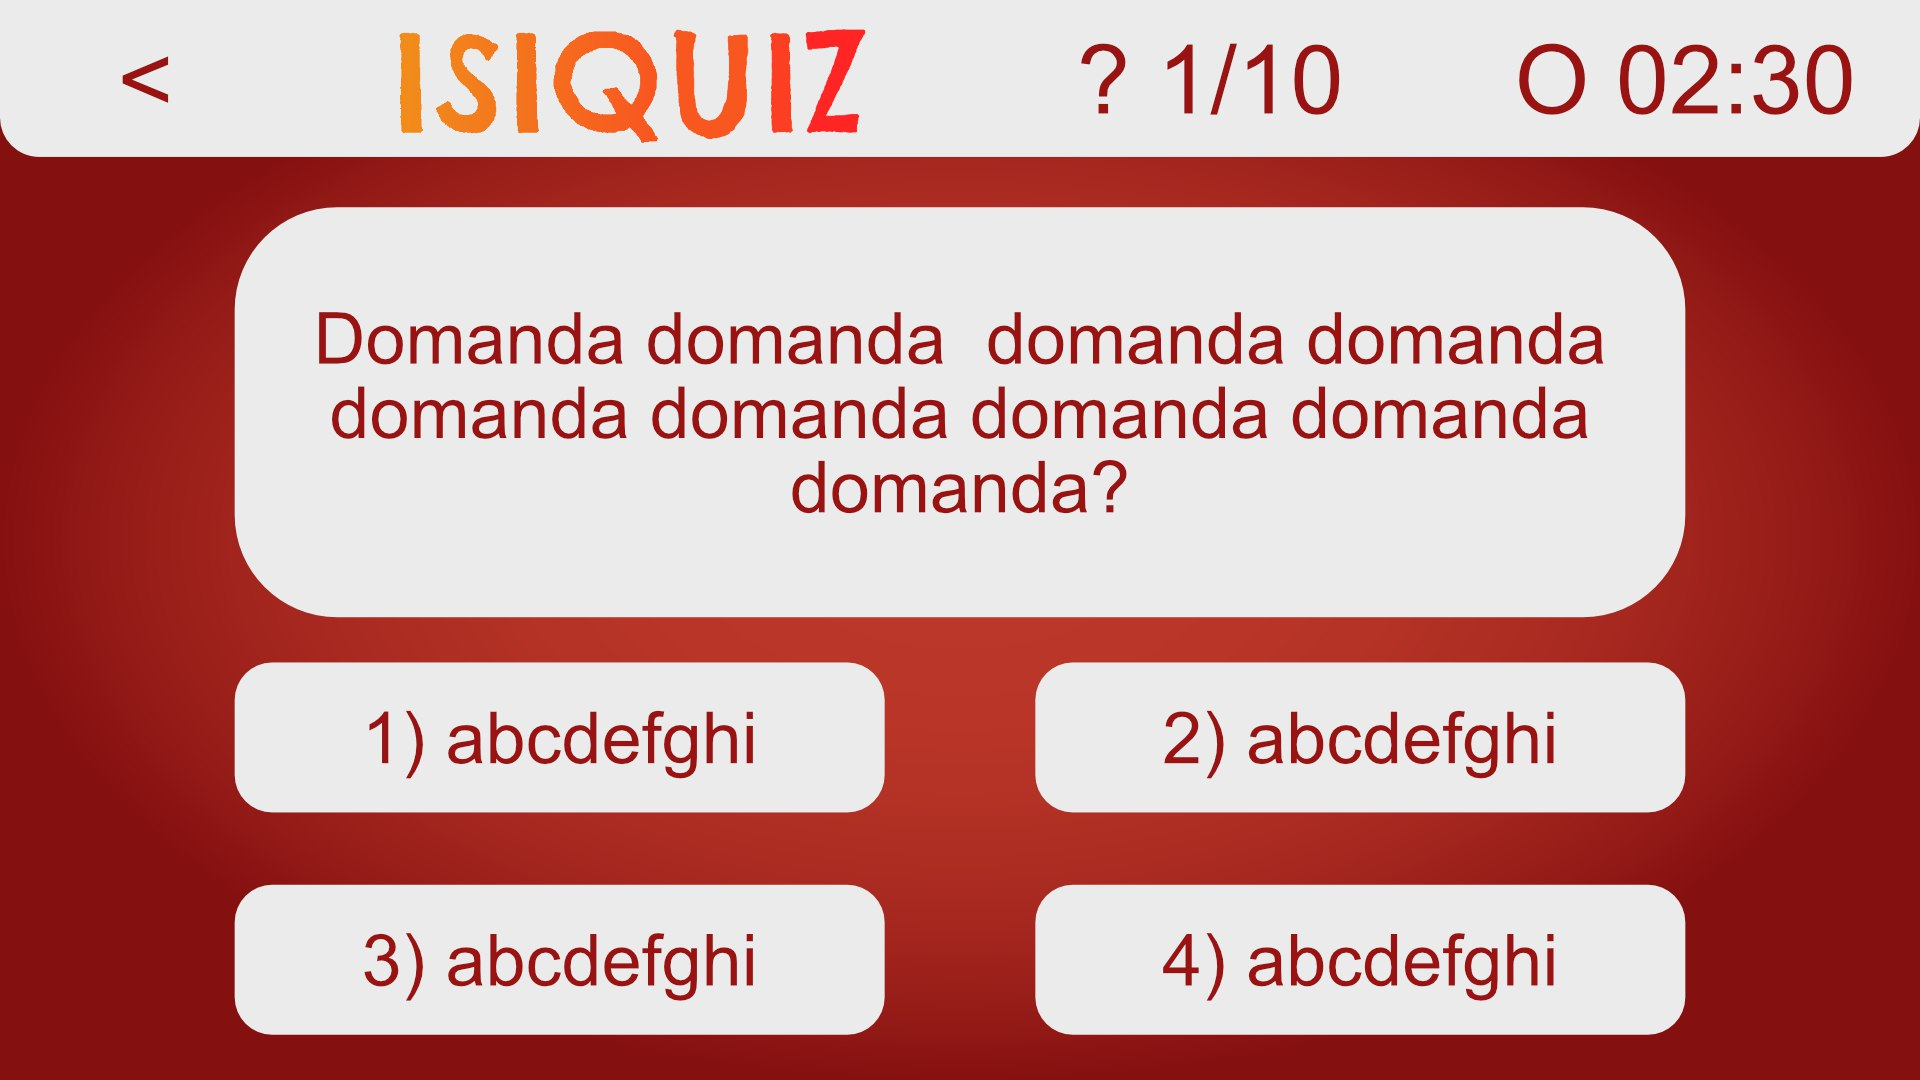
\includegraphics[width=\textwidth]{Images/mockup/quiz1.jpg}
            \caption{Quiz}
            \label{fig:Quiz1}
          \end{minipage}
          \hfill
          \begin{minipage}[b]{0.48\textwidth}
            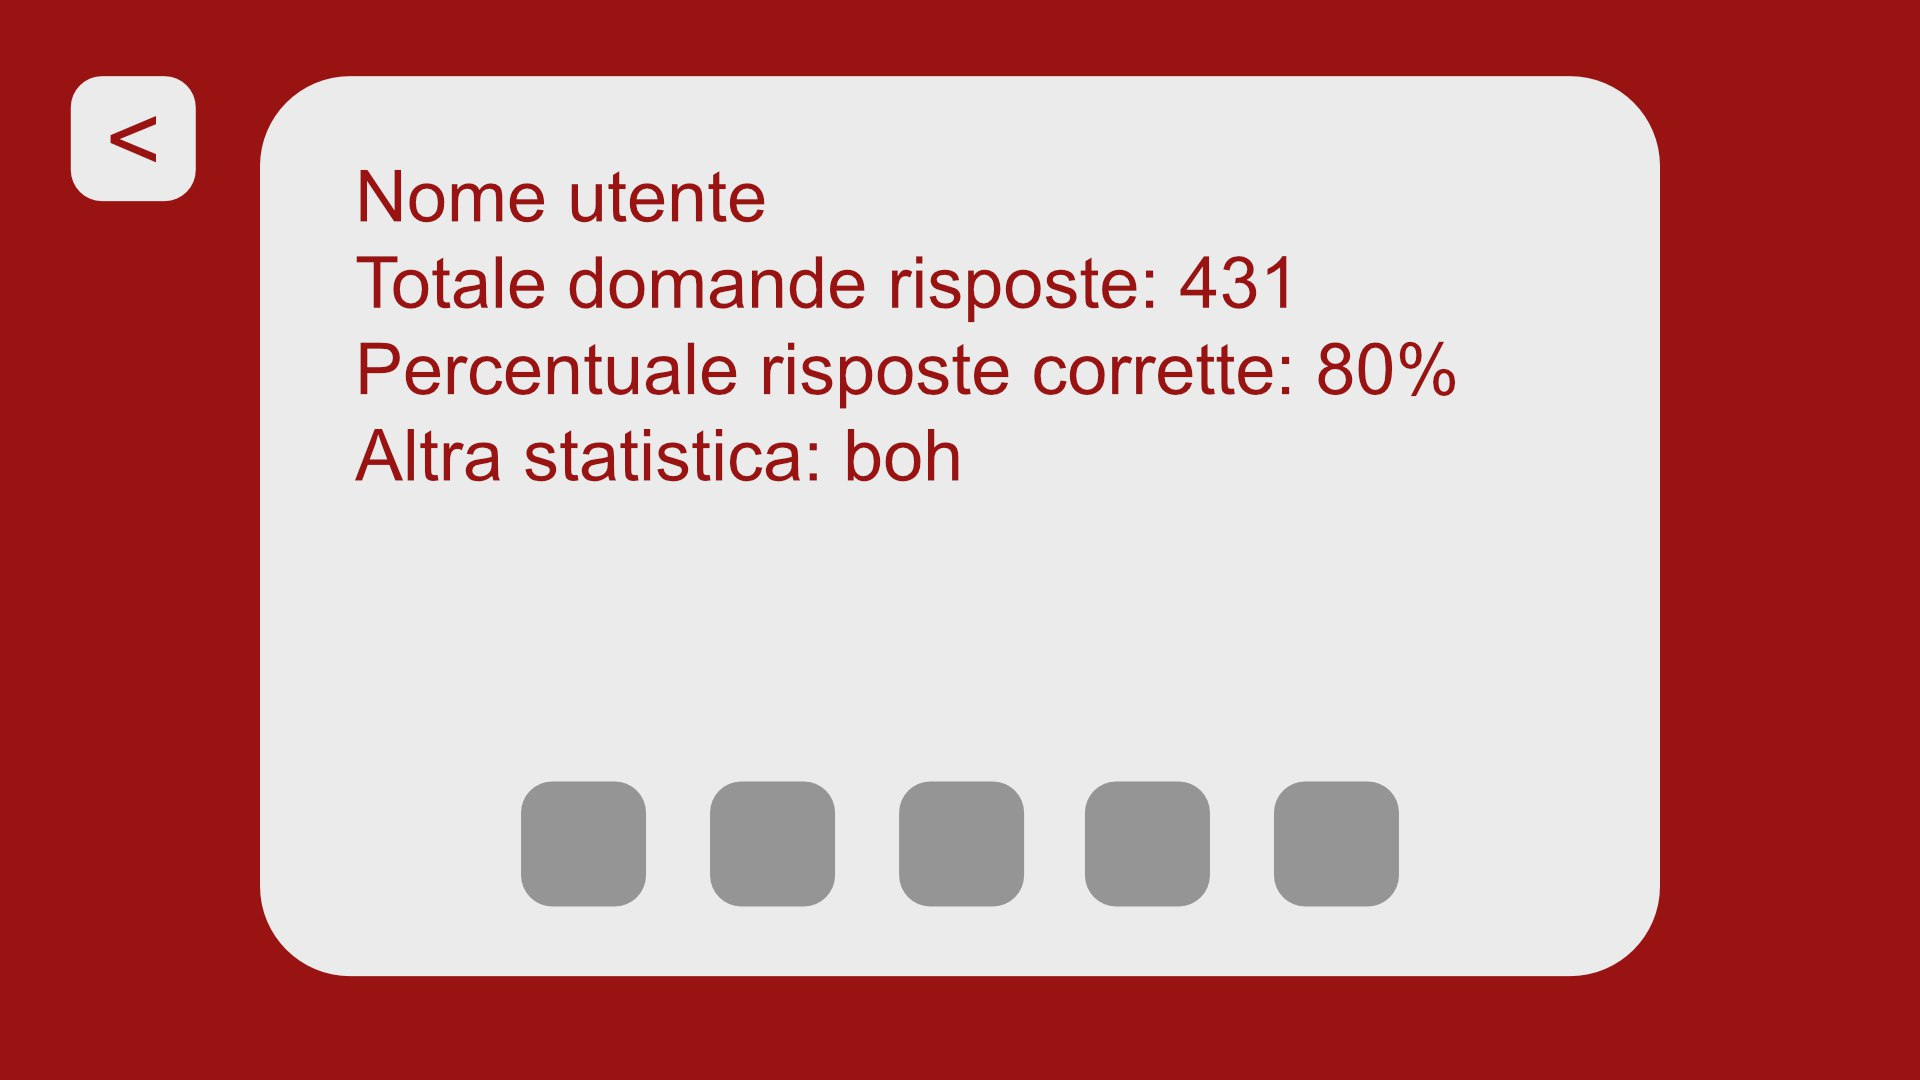
\includegraphics[width=\textwidth]{Images/mockup/achievements1.jpg}
            \caption{Statistiche di gioco e obiettivi raggiunti}
          \end{minipage}
        \end{figure}
          
        \begin{figure}[H]
          \centering
          \begin{minipage}[b]{0.48\textwidth}
            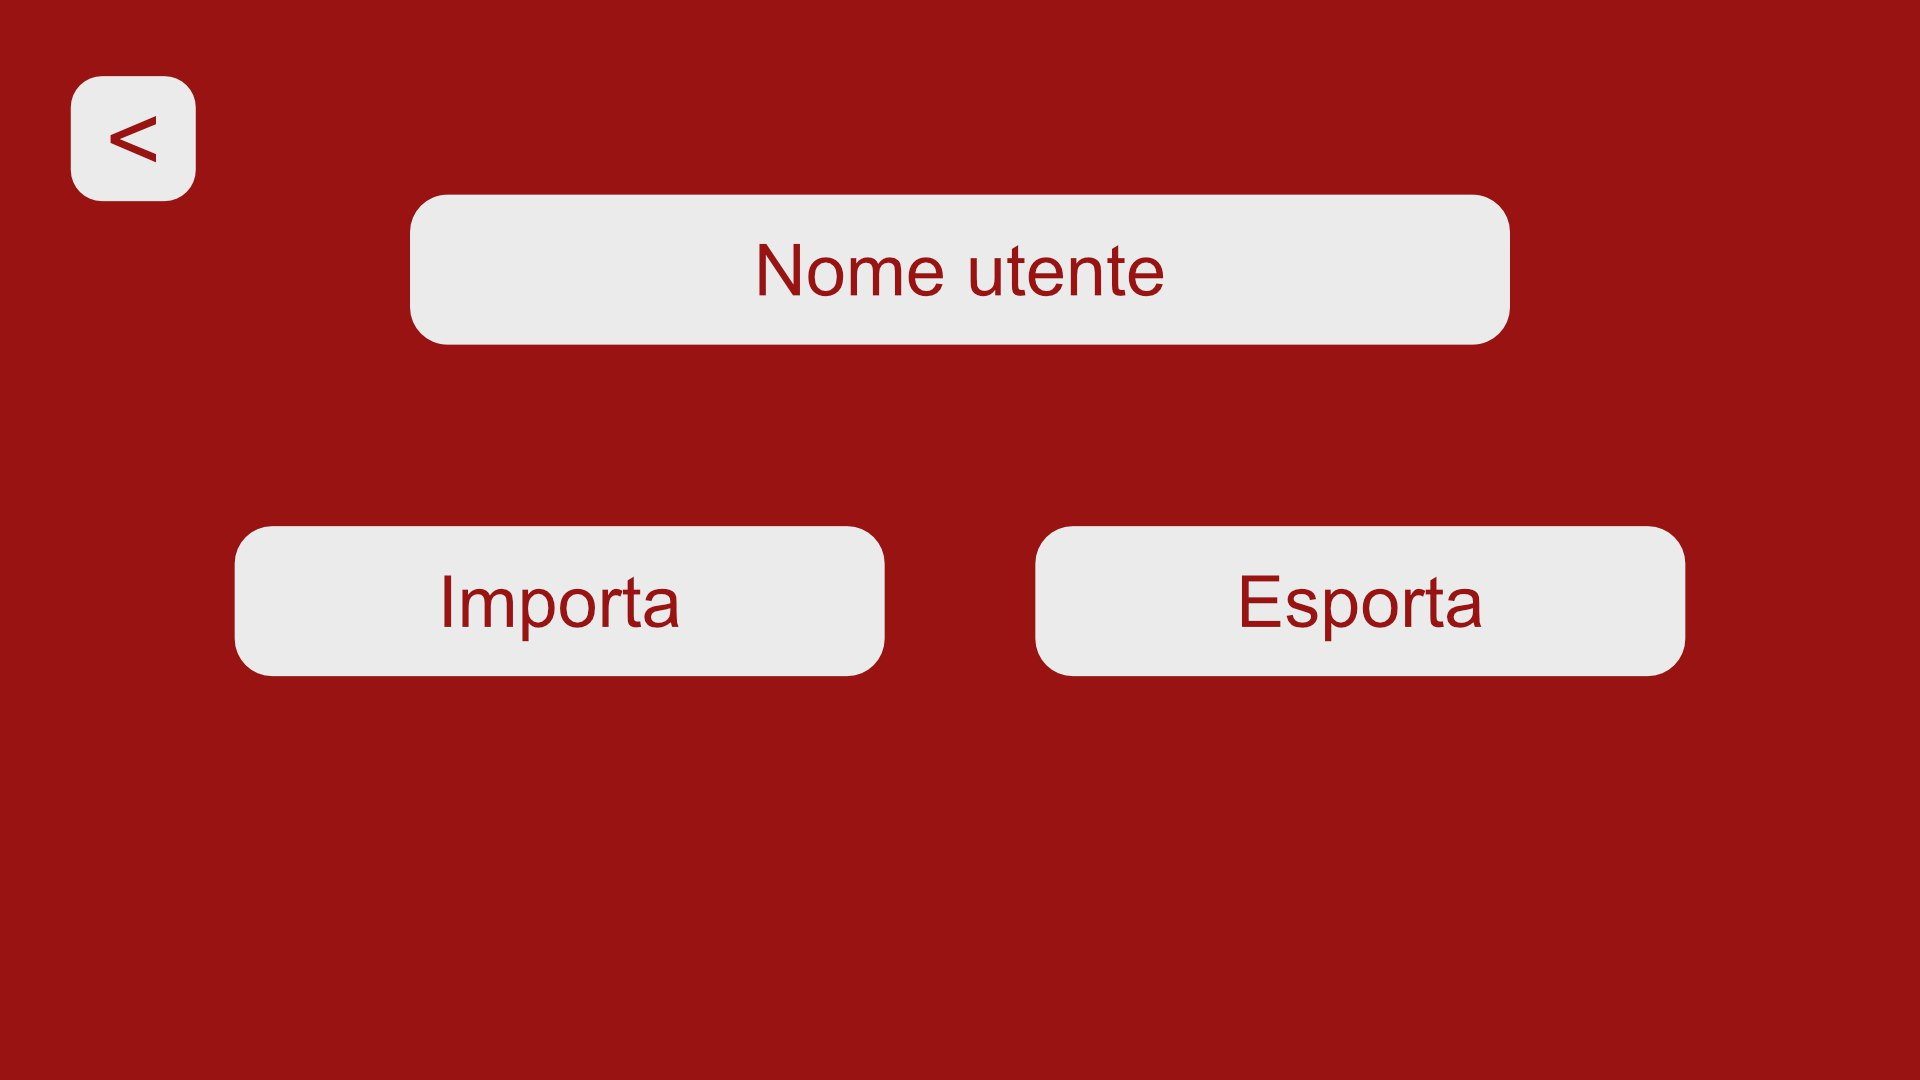
\includegraphics[width=\textwidth]{Images/mockup/settings1.jpg}
            \caption{Impostazioni Generali}
            \label{fig:Settings1}
          \end{minipage}
          \hfill
        \end{figure}
        
        \subsubsection{Mockup seconda versione}\label{mockup2}
        
        \begin{figure}[H]
          \centering
          \begin{minipage}[b]{0.48\textwidth}
            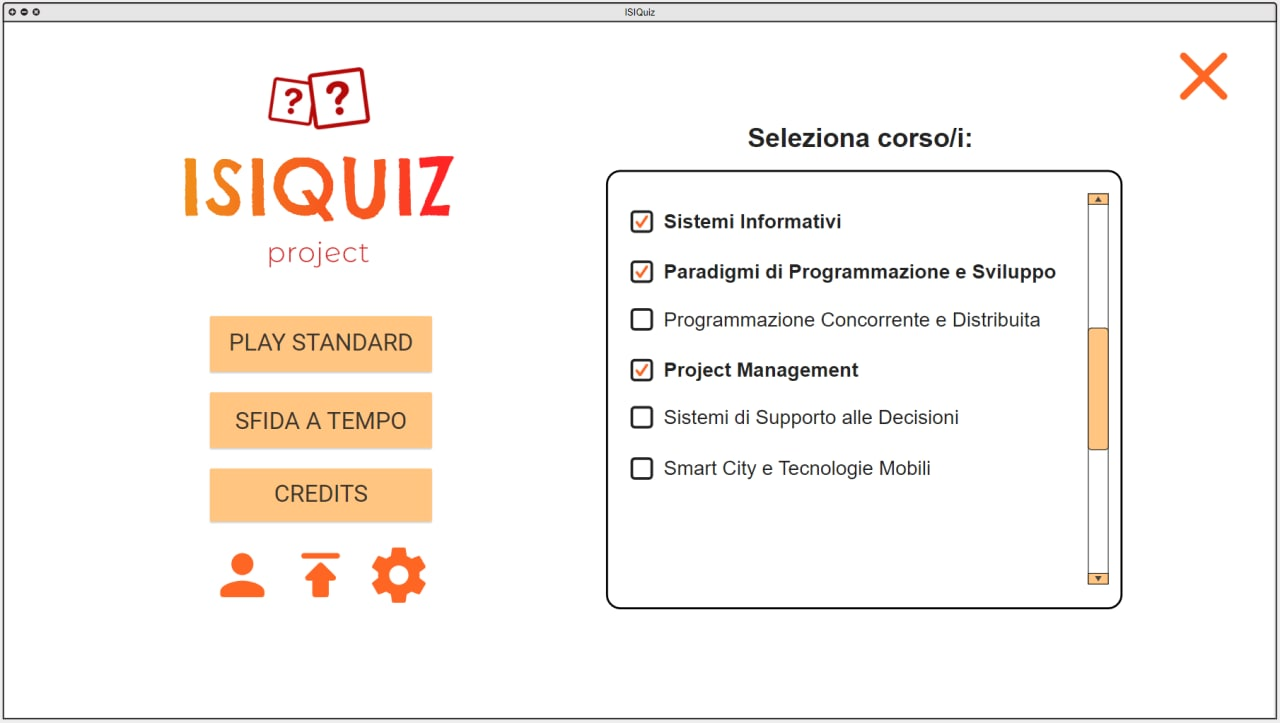
\includegraphics[width=\textwidth]{Images/mockup/home2.jpg}
            \caption{Pagina Iniziale}
            \label{fig:HomePage2}
          \end{minipage}
          \hfill
          \begin{minipage}[b]{0.48\textwidth}
            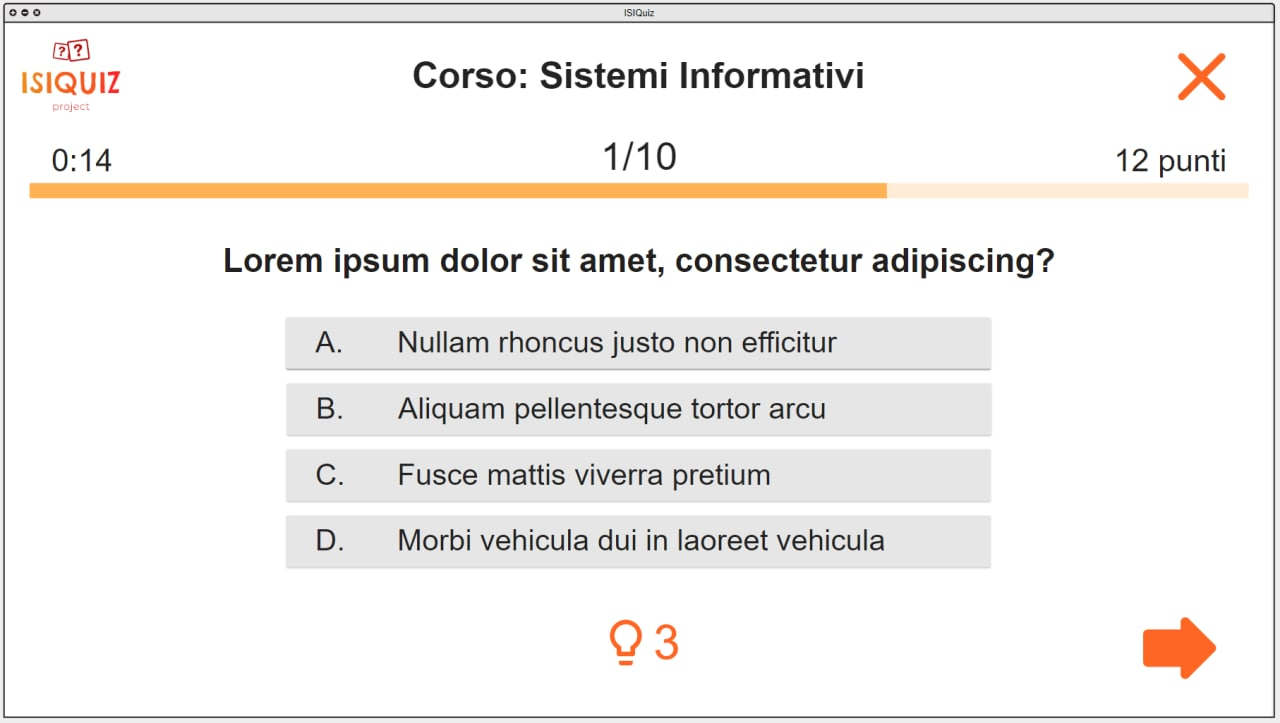
\includegraphics[width=\textwidth]{Images/mockup/quiz2.jpg}
            \caption{Quiz}
            \label{fig:Quiz2}
          \end{minipage}
        \end{figure}
          
        \begin{figure}[H]
          \centering
          \begin{minipage}[b]{0.48\textwidth}
            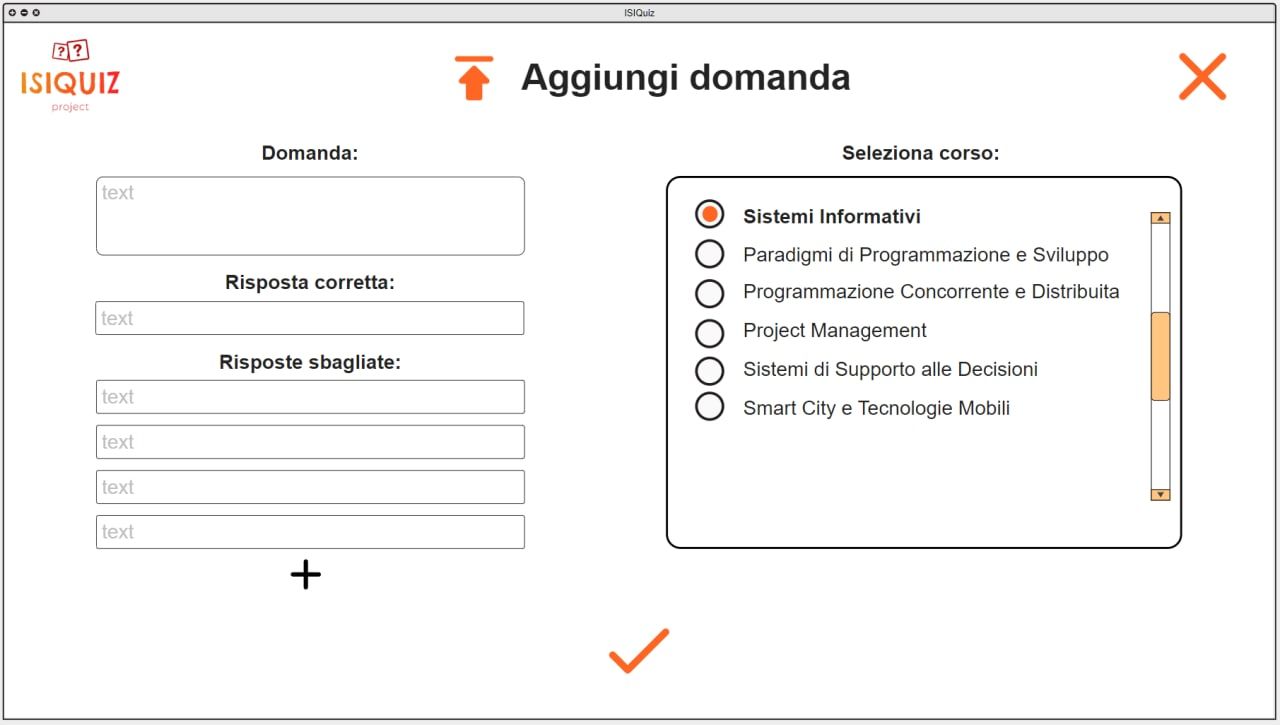
\includegraphics[width=\textwidth]{Images/mockup/import2.jpg}
            \caption{Inserimento di nuove domande e relative risposte per un determinato corso}
            \label{fig:Import2}
          \end{minipage}
          \hfill
        \end{figure}
        
        \subsubsection{Mockup definitivi}\label{mockupFinished}
        
        \begin{figure}[H]
          \centering
          \begin{minipage}[b]{0.48\textwidth}
            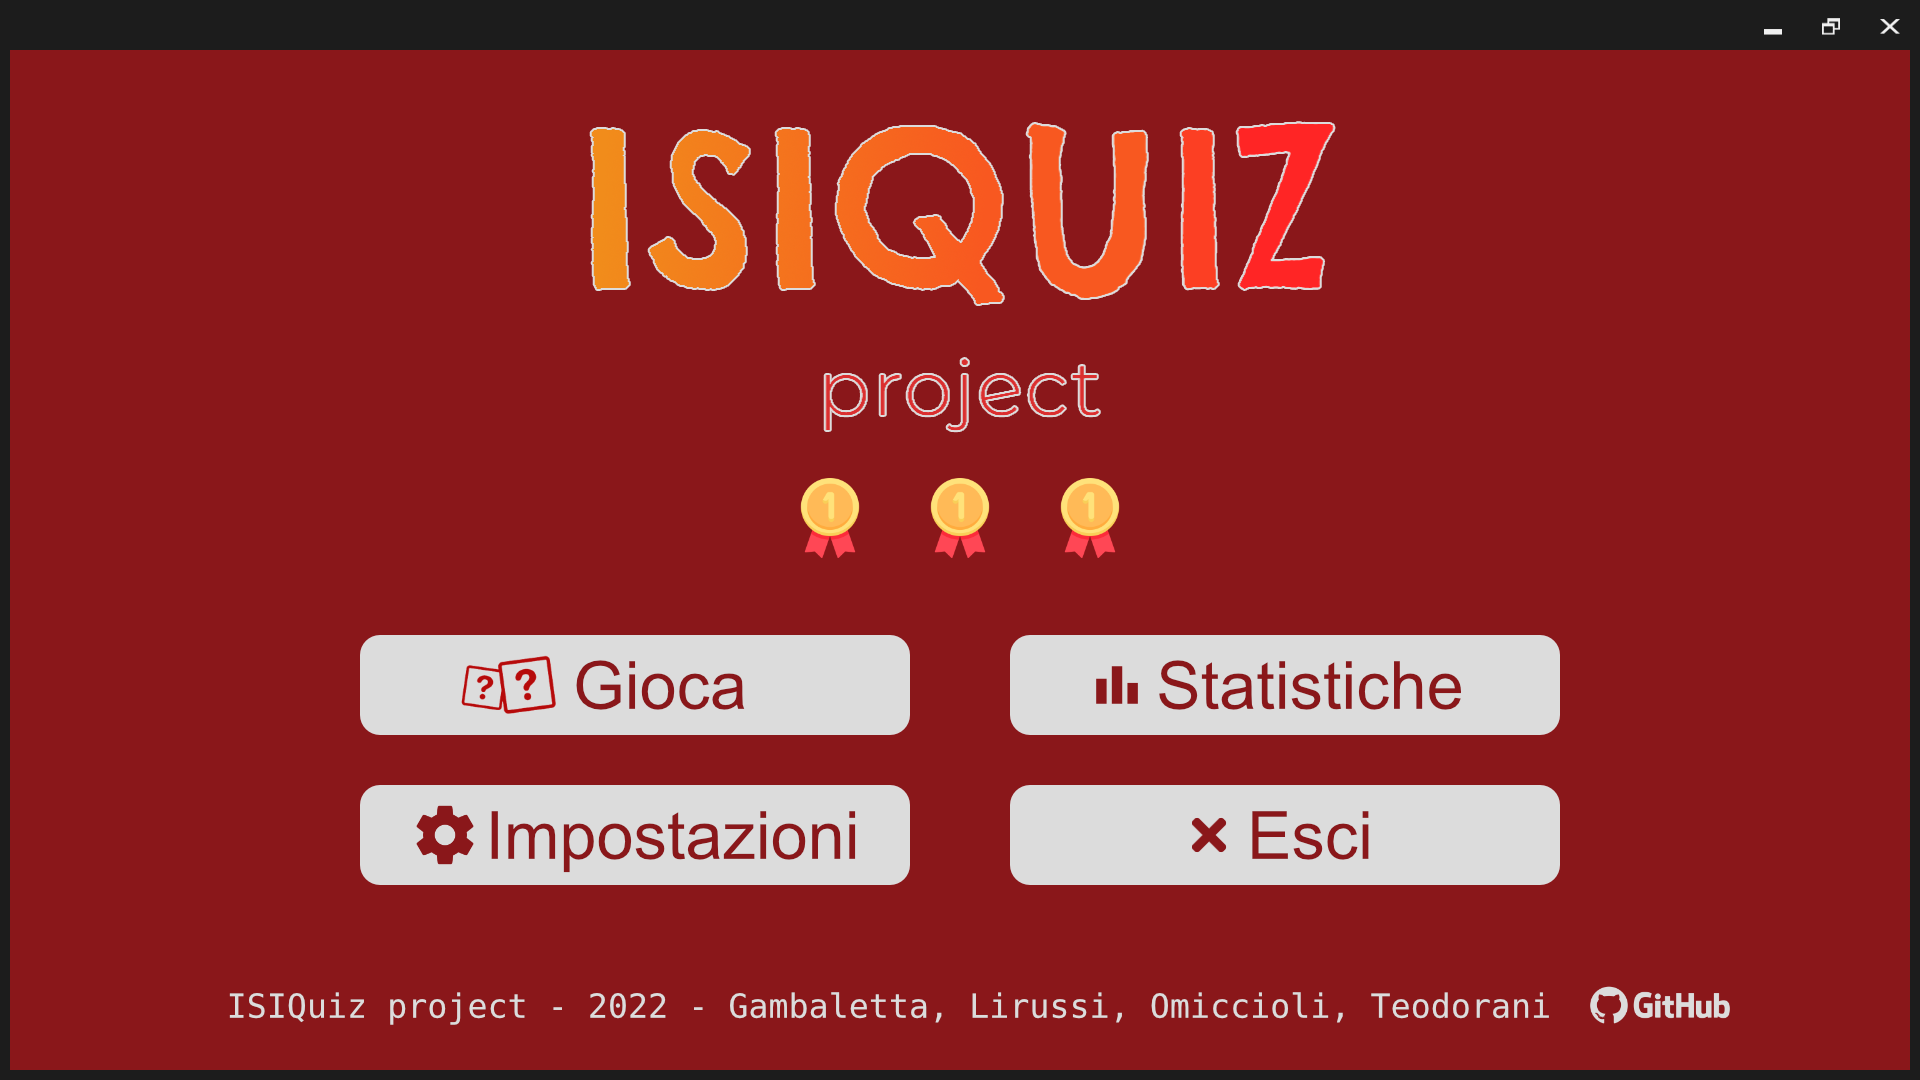
\includegraphics[width=\textwidth]{Images/mockup/home3.png}
            \caption{Pagina iniziale}
            \label{fig:home3}
          \end{minipage}
          \hfill
          \begin{minipage}[b]{0.48\textwidth}
            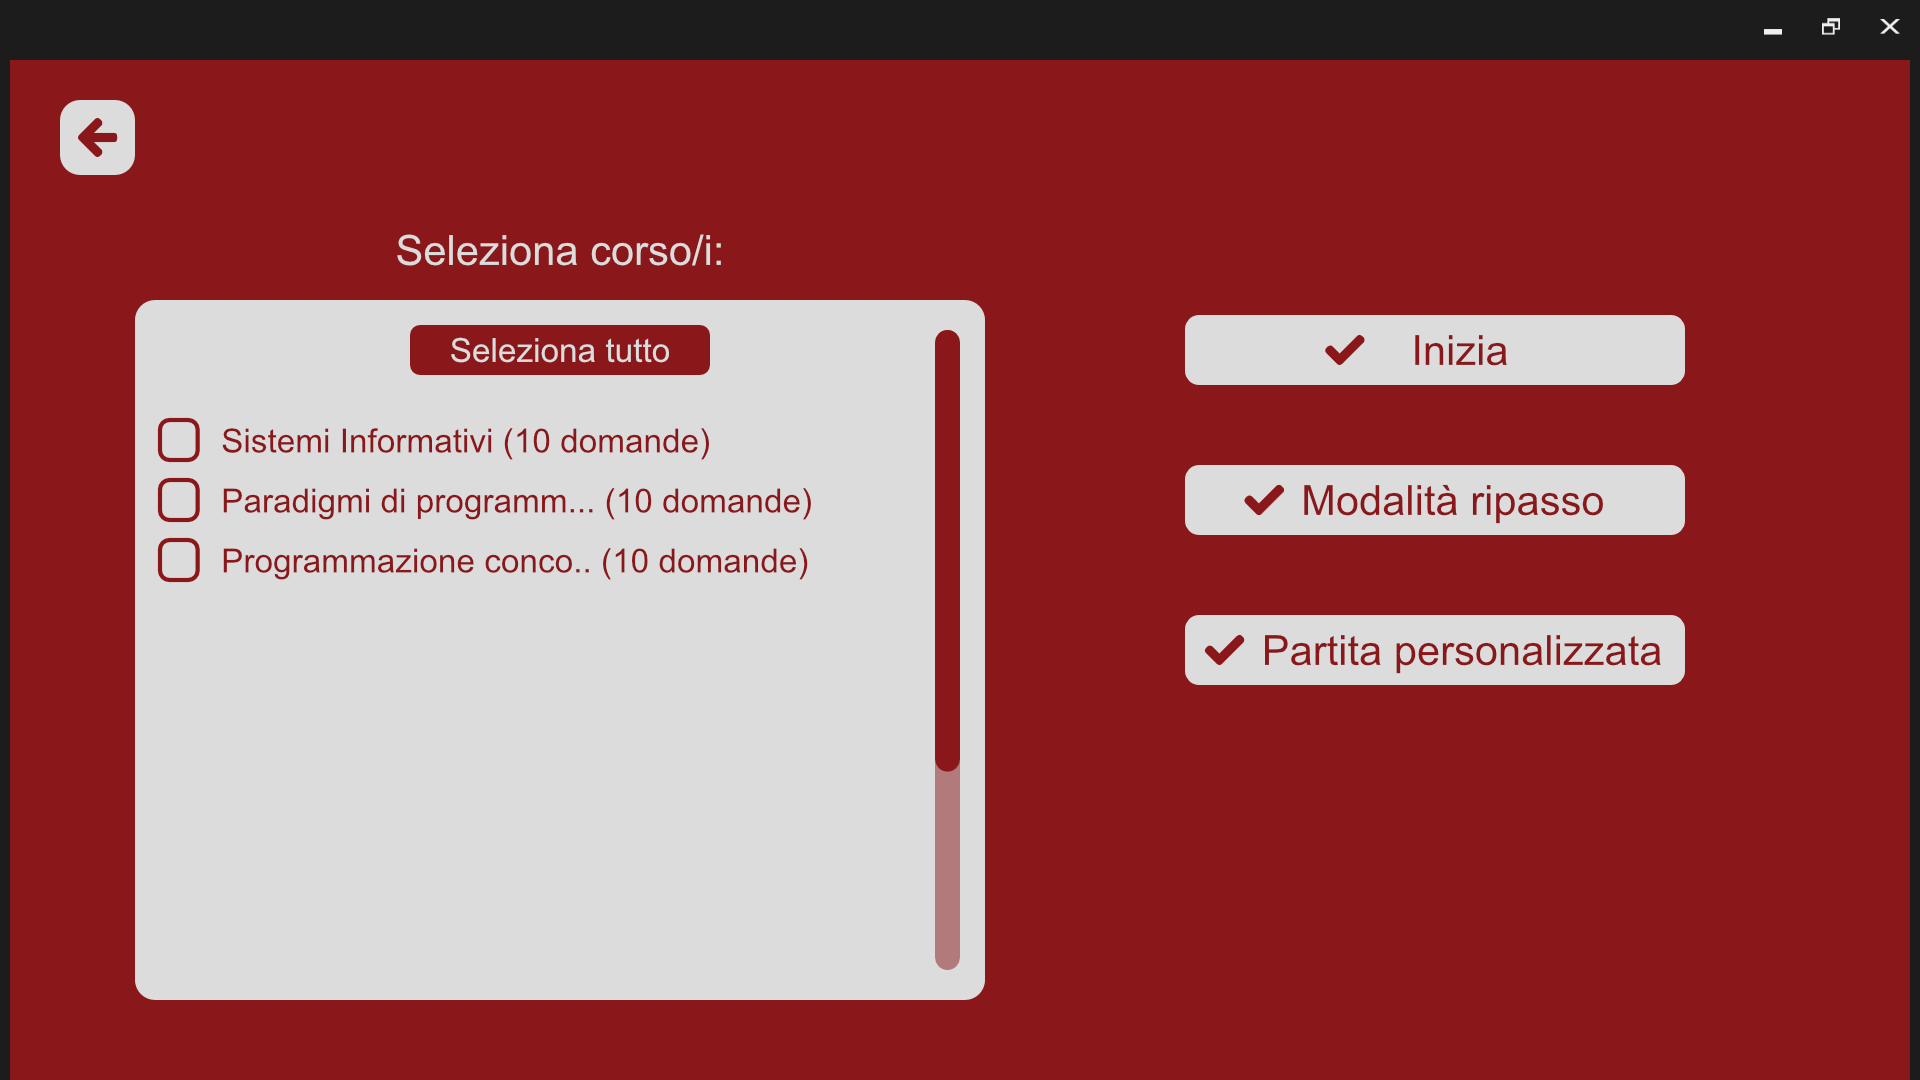
\includegraphics[width=\textwidth]{Images/mockup/start3.png}
            \caption{Settaggio di una partita prima di iniziarla}
            \label{fig:start3}
          \end{minipage}
        \end{figure}

        \begin{figure}[H]
          \centering
          \begin{minipage}[b]{0.48\textwidth}
            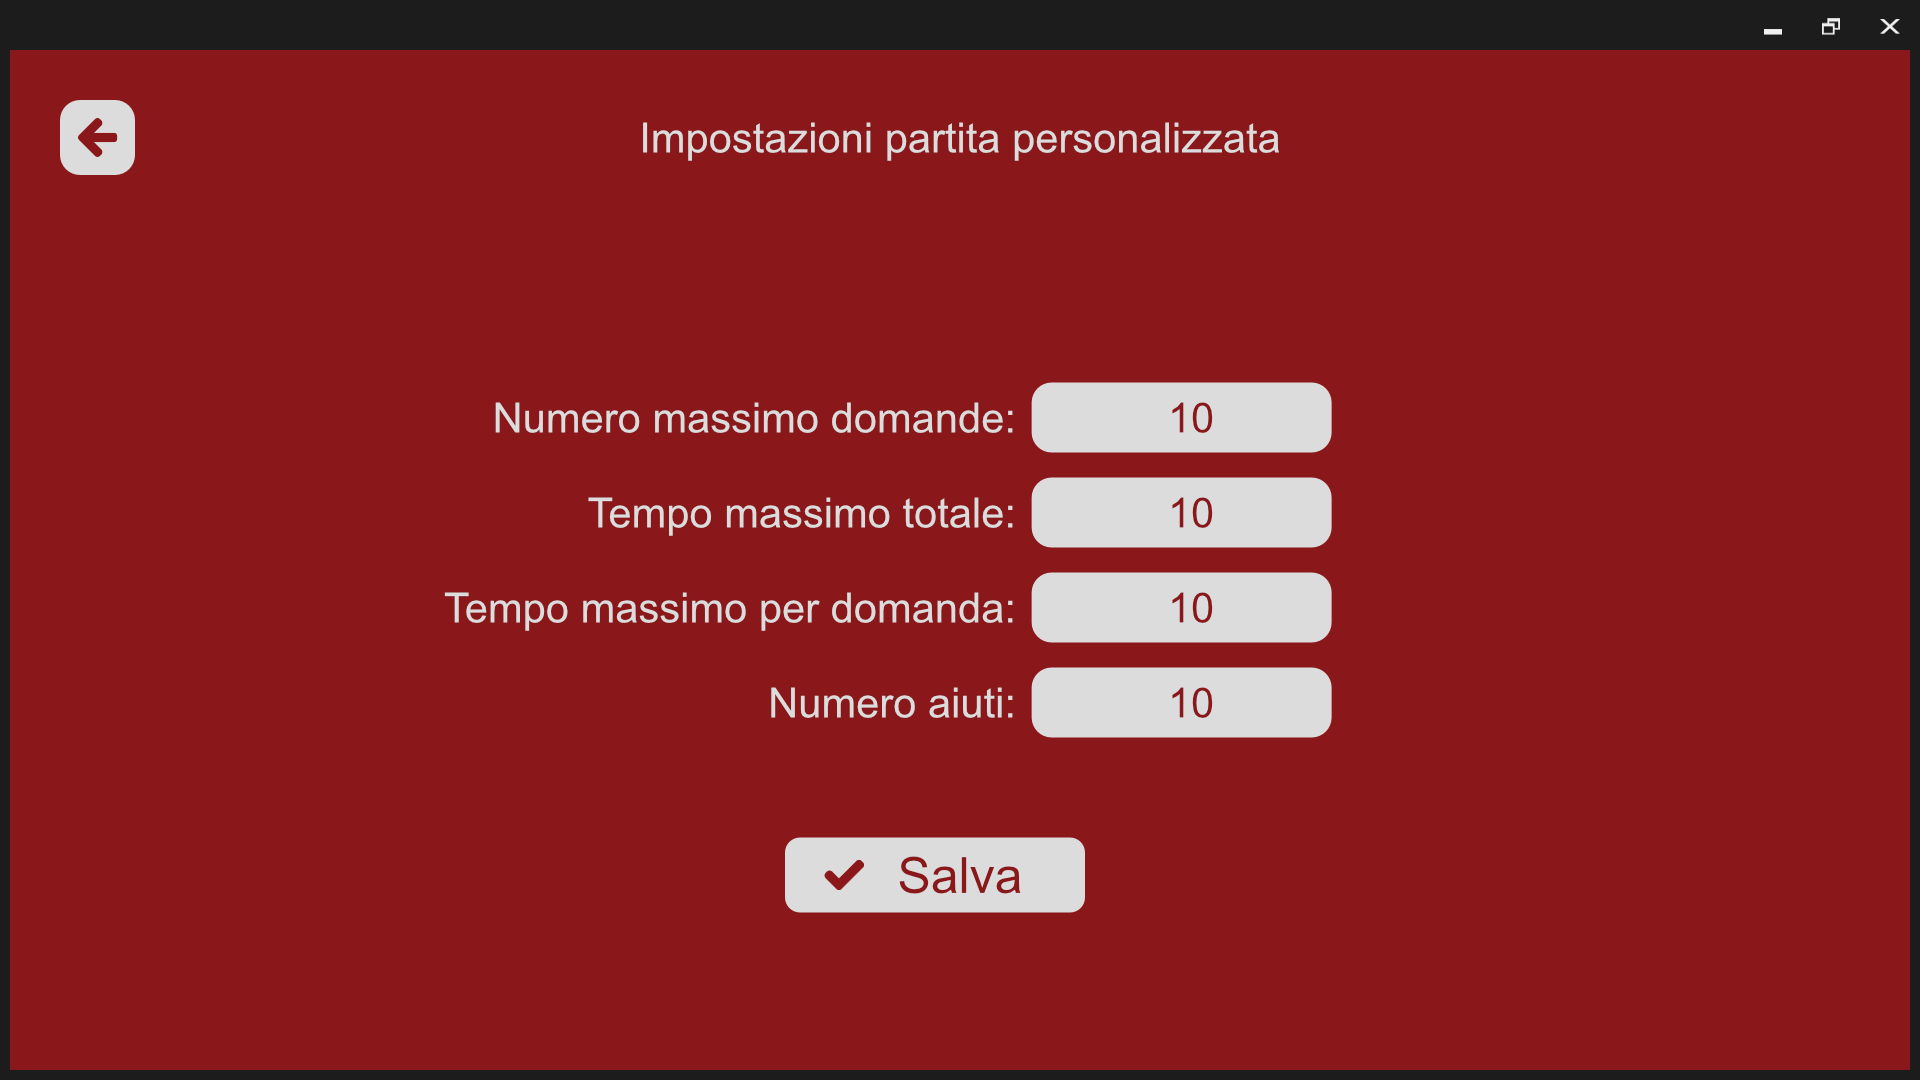
\includegraphics[width=\textwidth]{Images/mockup/custom.png}
            \caption{Settaggio parametri per una partita personalizzata}
            \label{fig:custom}
          \end{minipage}
          \hfill
          \begin{minipage}[b]{0.48\textwidth}
            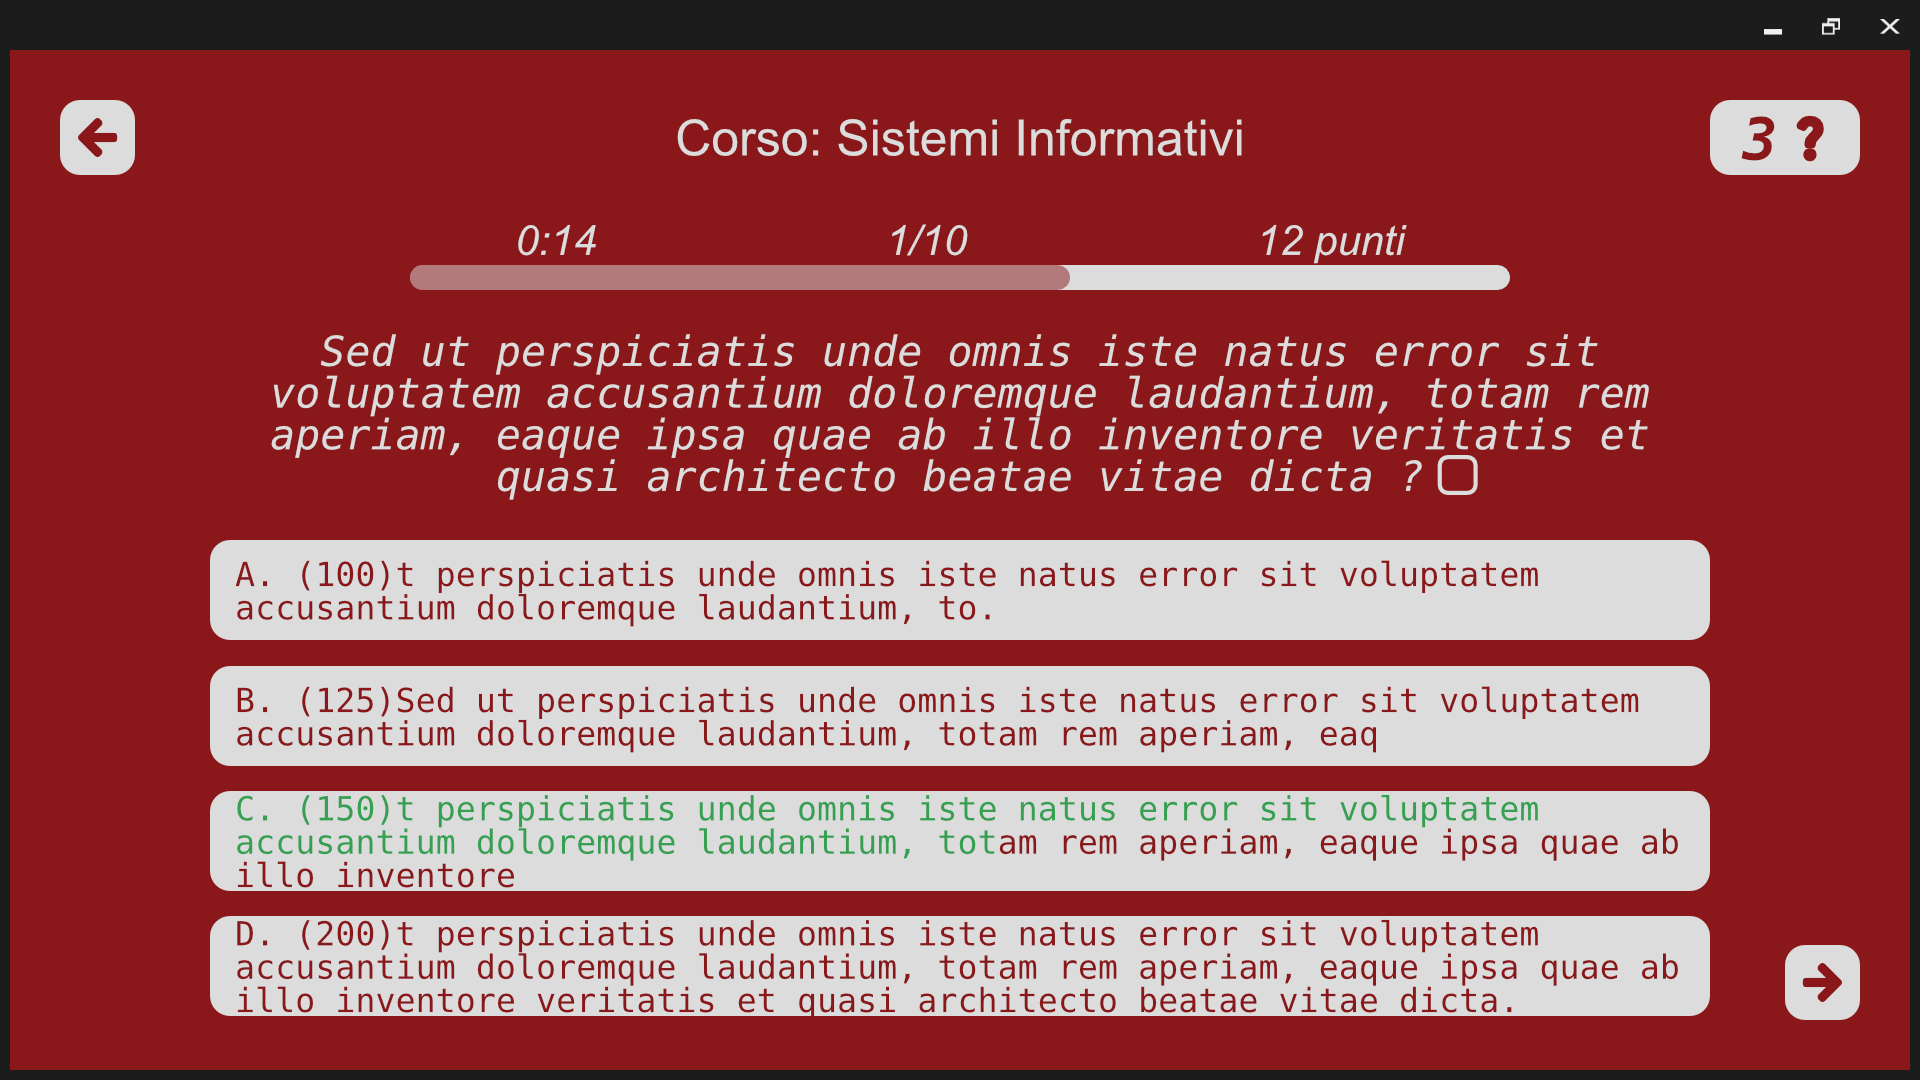
\includegraphics[width=\textwidth]{Images/mockup/quiz3.png}
            \caption{Quiz}
            \label{fig:quiz3}
          \end{minipage}
        \end{figure}

        \begin{figure}[H]
          \centering
          \begin{minipage}[b]{0.48\textwidth}
             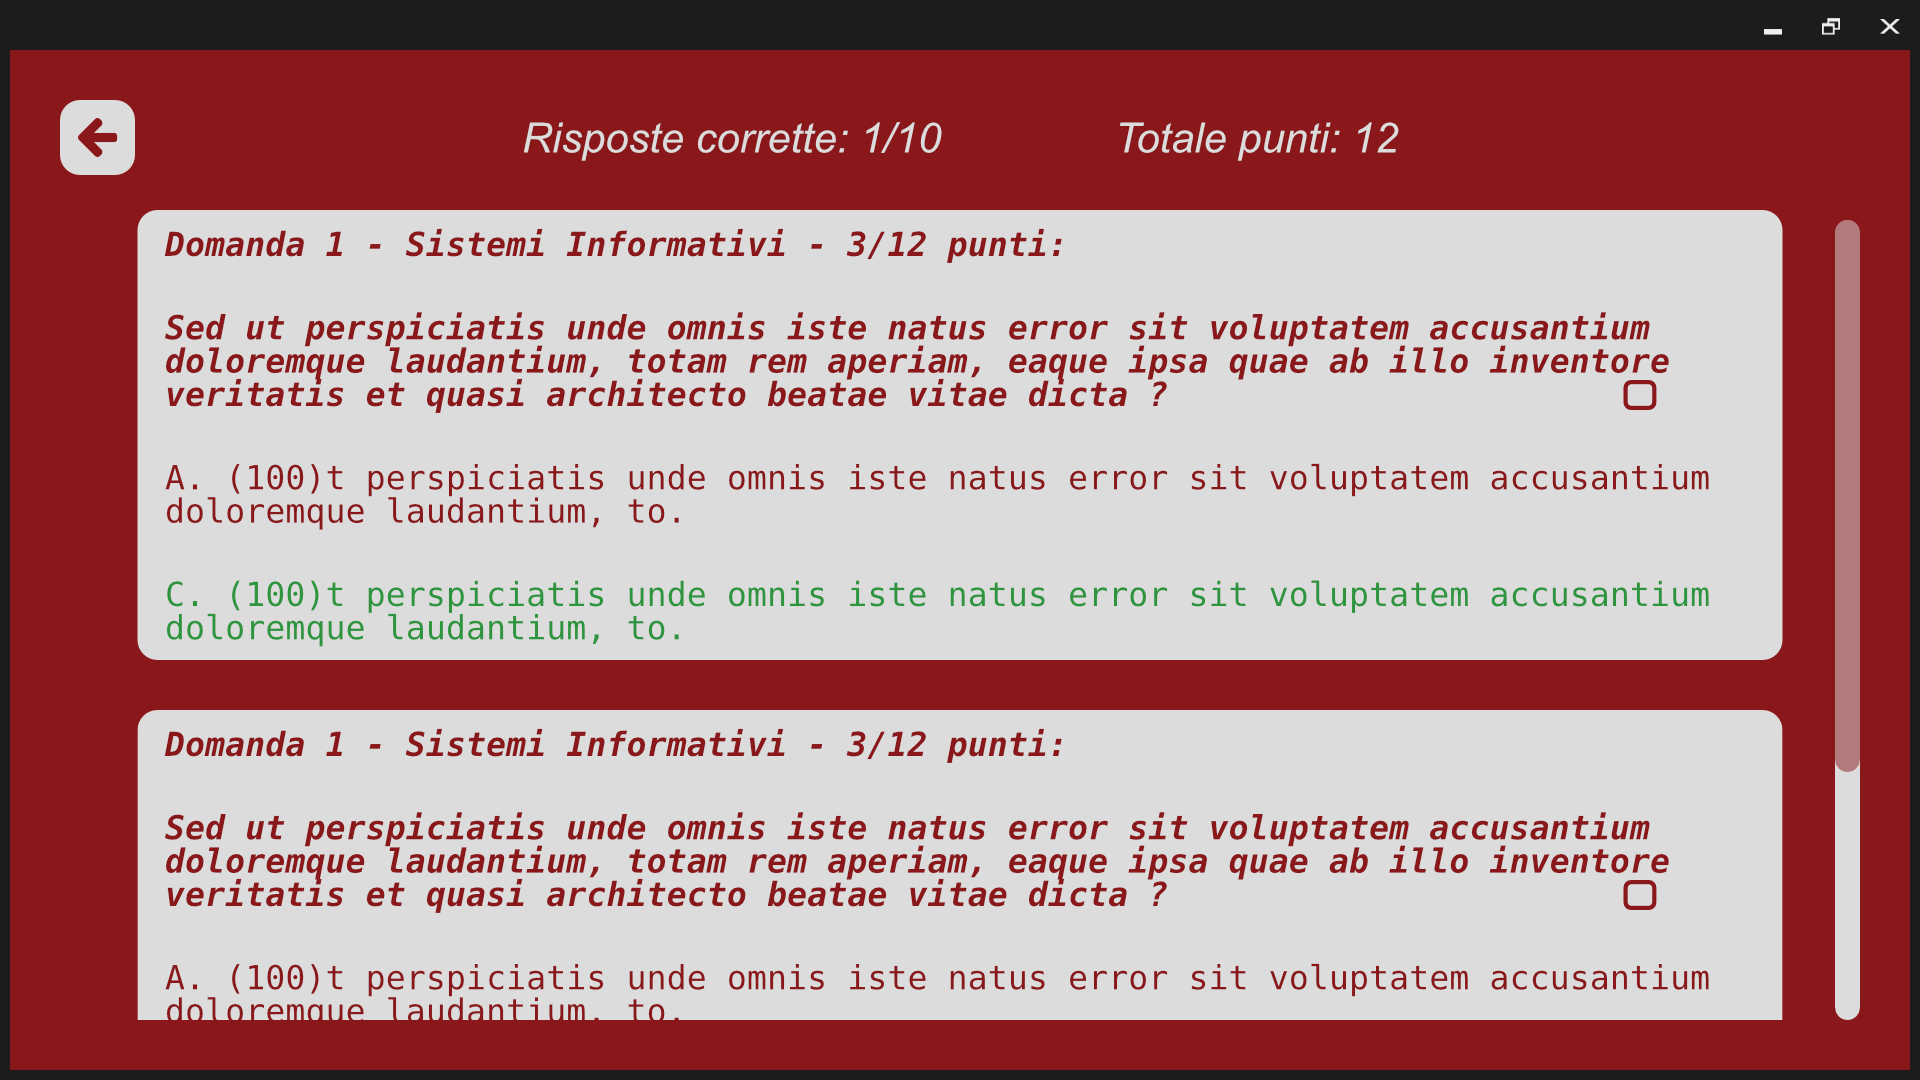
\includegraphics[width=\textwidth]{Images/mockup/review.png}
            \caption{Revisione al termine di un quiz}
            \label{fig:review}
          \end{minipage}
          \hfill
          \begin{minipage}[b]{0.48\textwidth}
            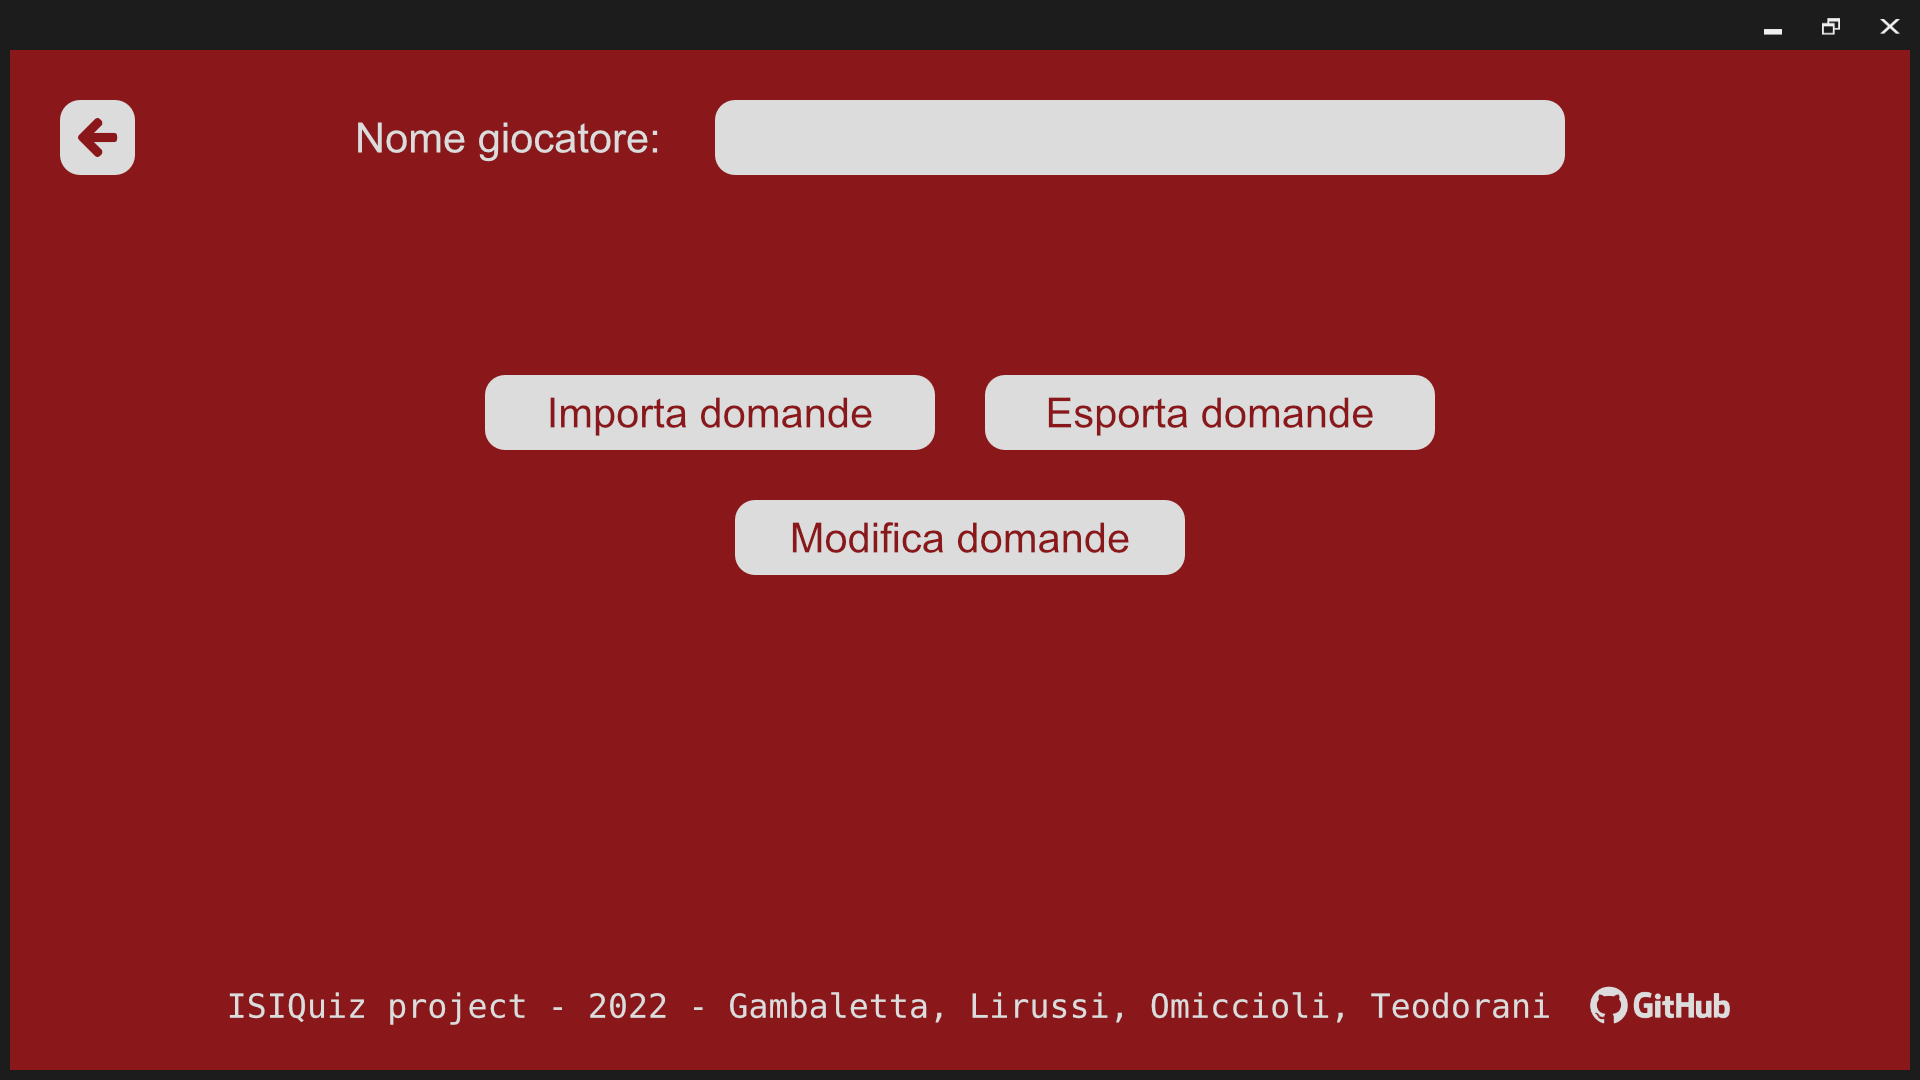
\includegraphics[width=\textwidth]{Images/mockup/settings3.png}
            \caption{Impostazioni generali}
            \label{fig:settings3}
          \end{minipage}
        \end{figure}

        \begin{figure}[H]
          \centering
          \begin{minipage}[b]{0.48\textwidth}
            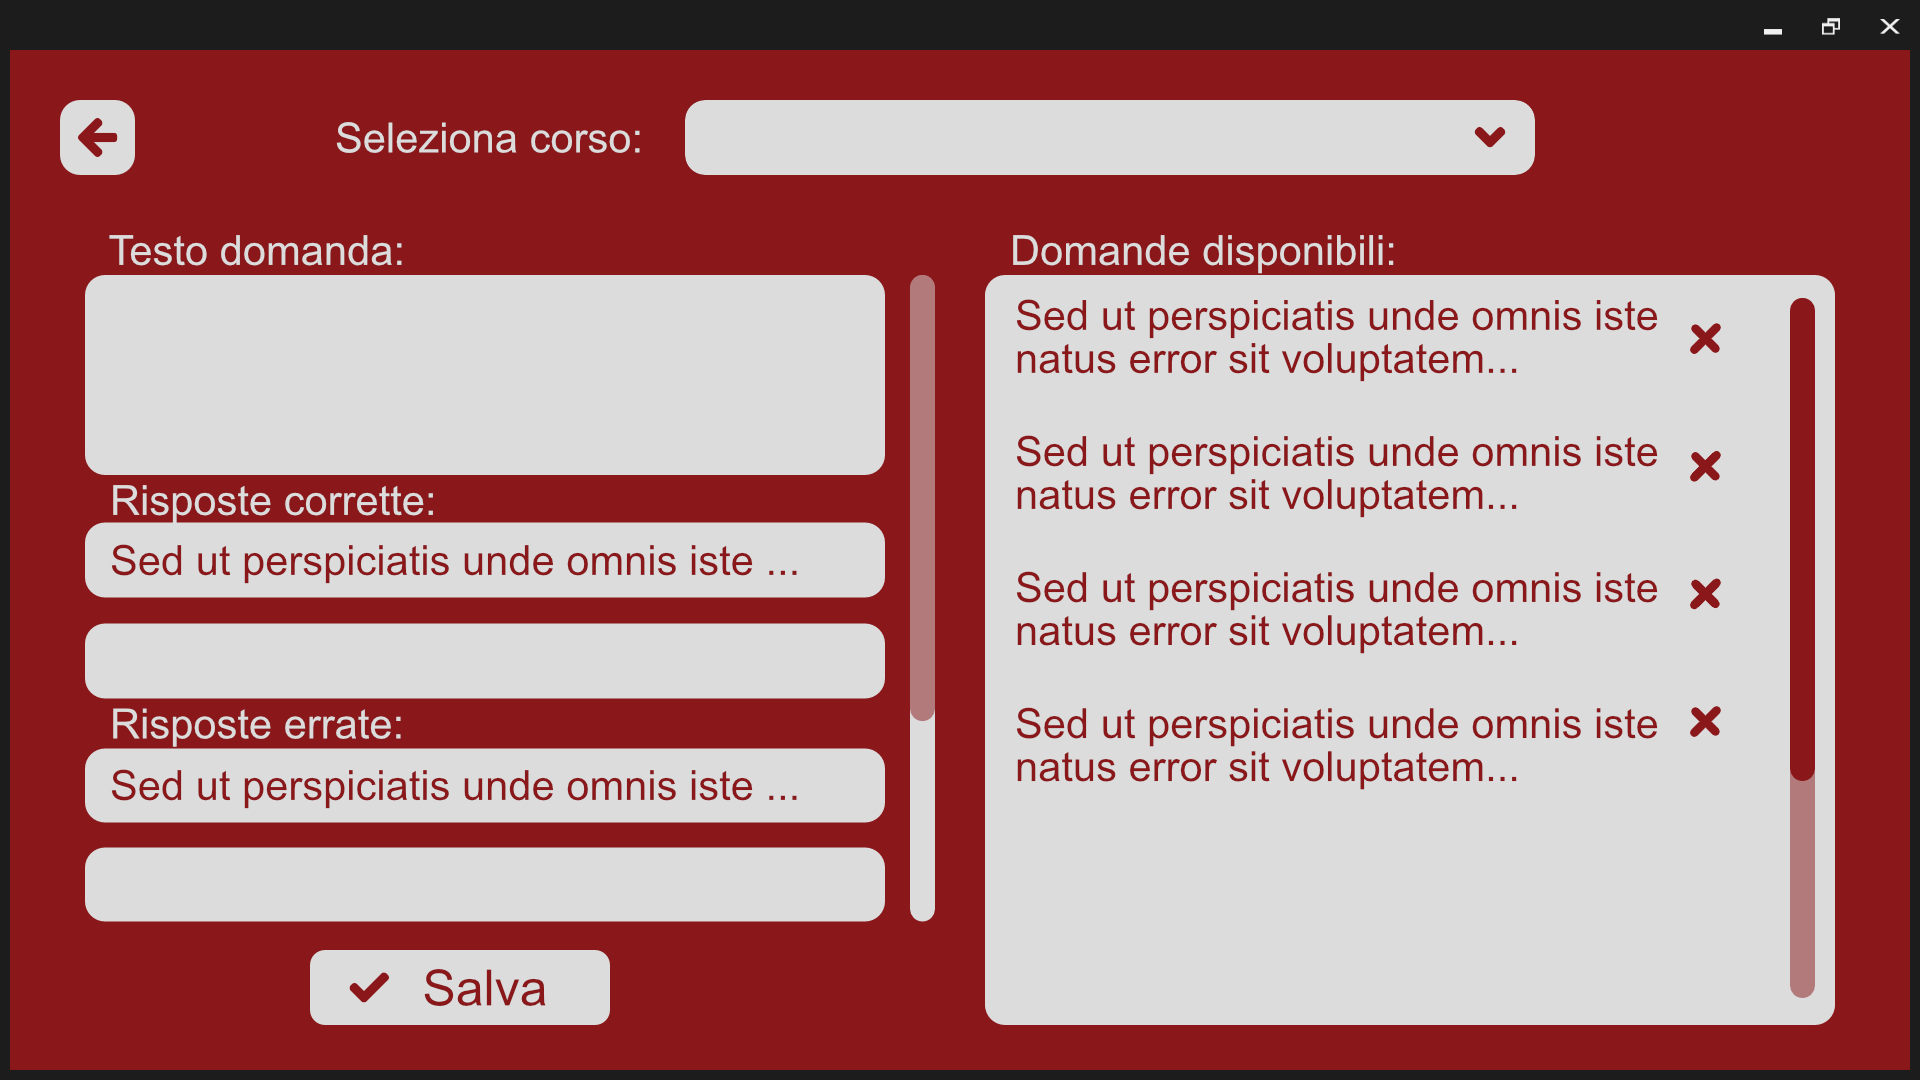
\includegraphics[width=\textwidth]{Images/mockup/import3.png}
            \caption{Inserimento di nuove domande e relative risposte per un determinato corso}
            \label{fig:import3}
          \end{minipage}
          \hfill
          \begin{minipage}[b]{0.48\textwidth}
            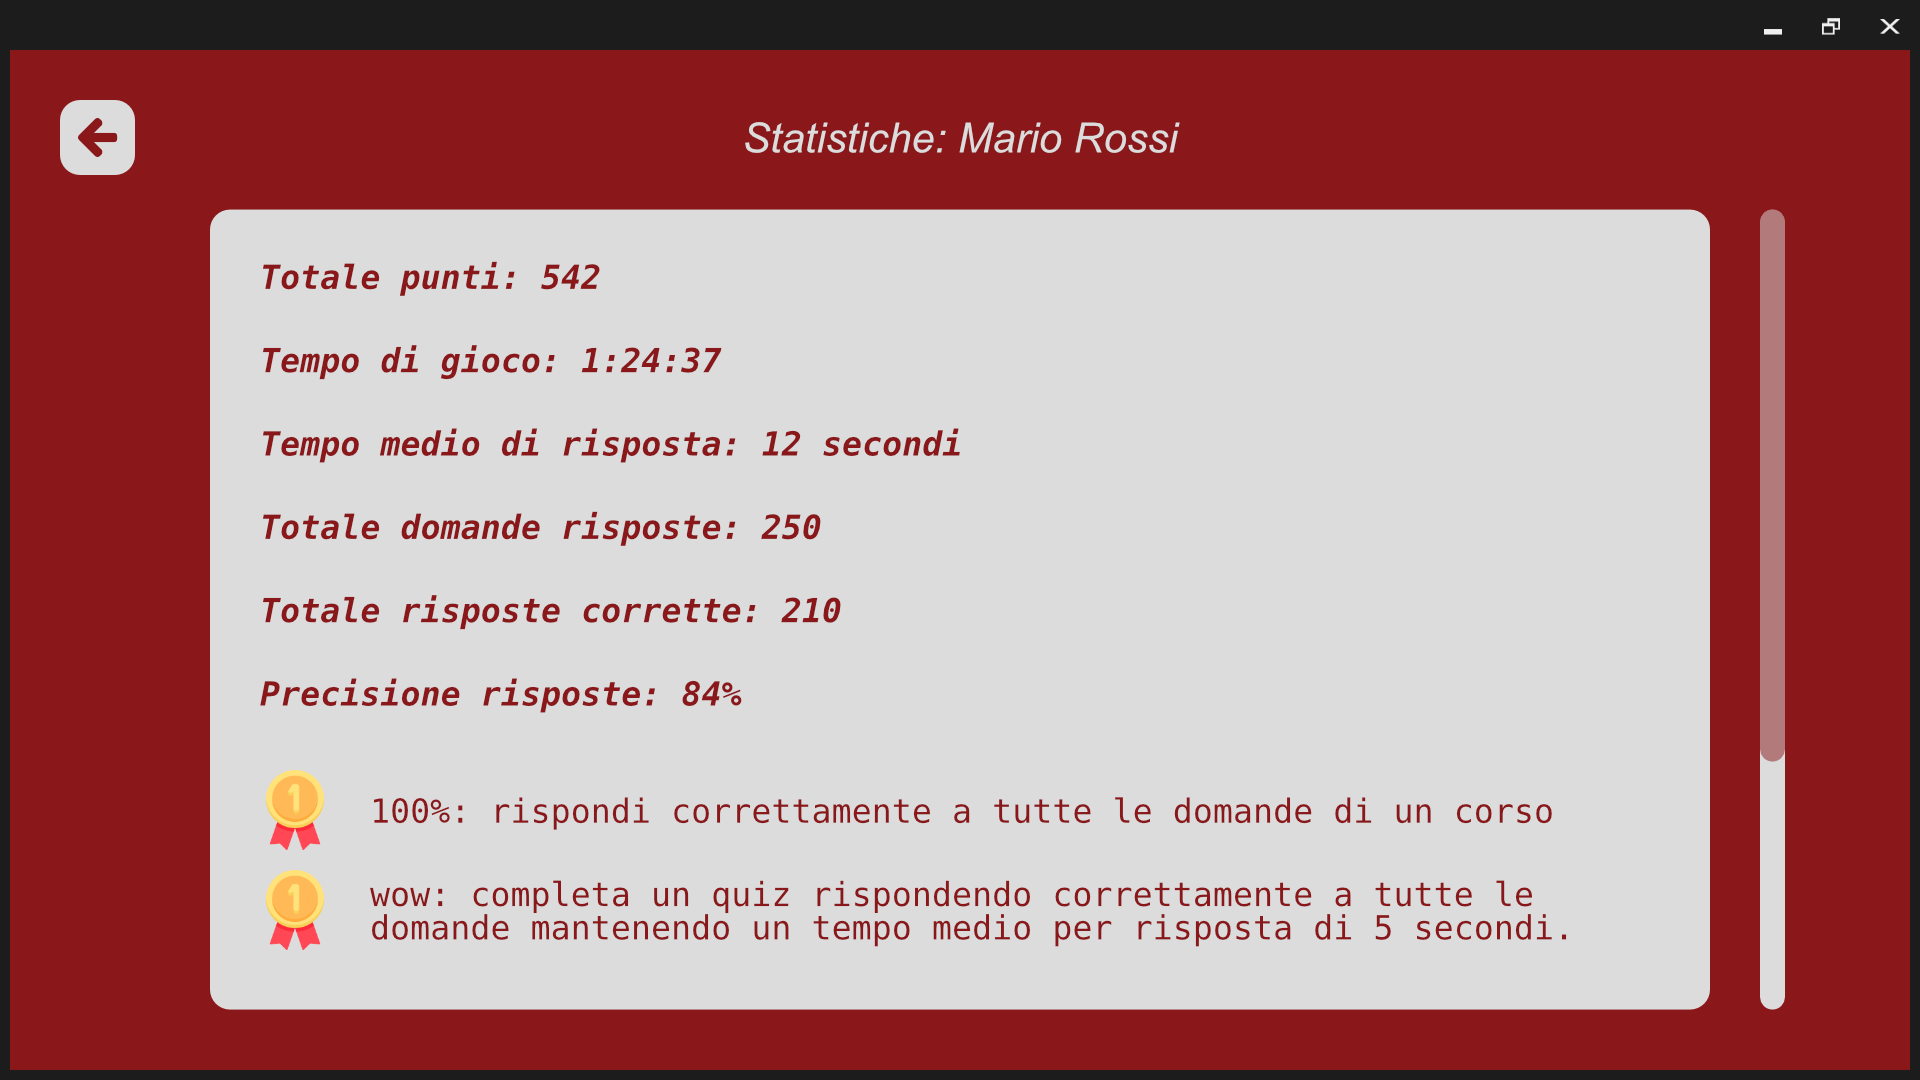
\includegraphics[width=\textwidth]{Images/mockup/achievements3.png}
            \caption{Statistiche di gioco e obiettivi raggiunti}
            \label{fig:achievements3}
          \end{minipage}
        \end{figure}

        \begin{figure}[H]
            \centering
            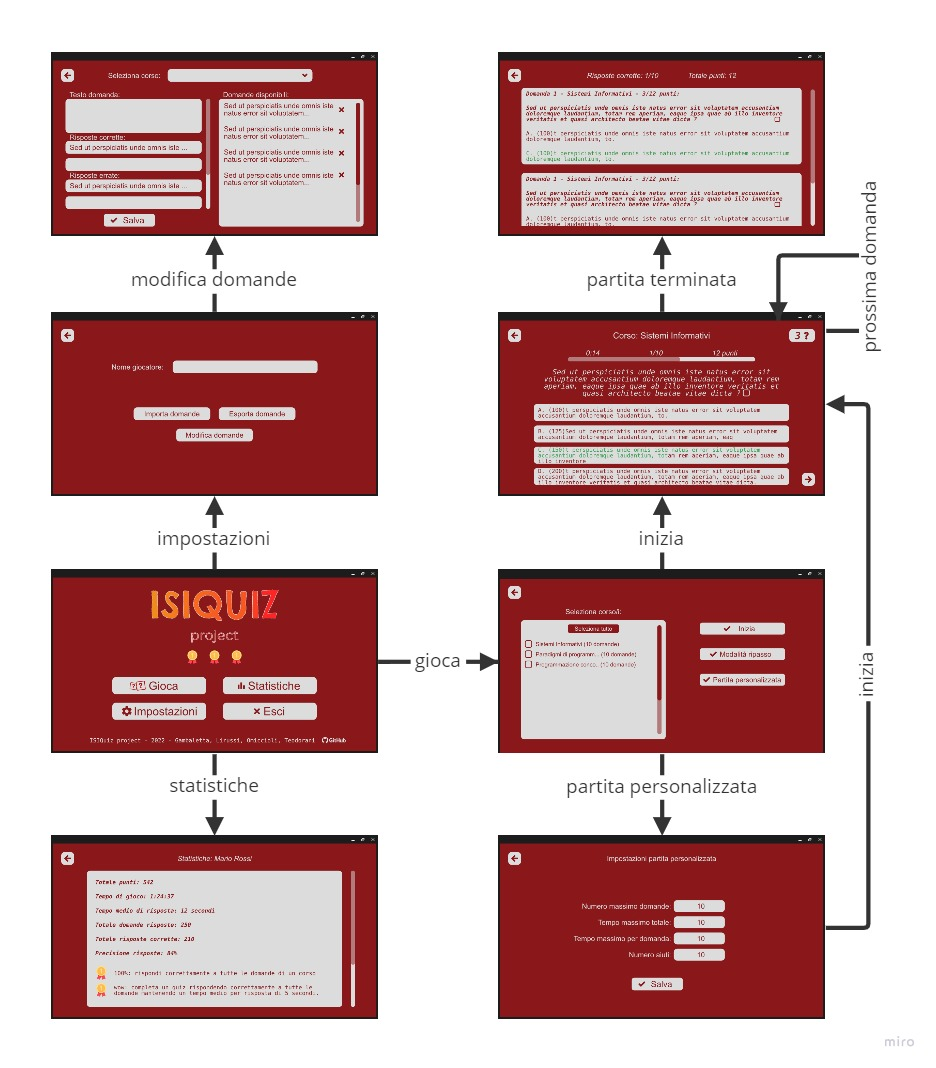
\includegraphics[width=\textwidth]{Miro/mockup_navigation.jpg}
            \caption{Tutti i mockup dell'applicazione con navigazione tra le pagine}
            \label{fig:mockup_nav}
        \end{figure}
	    
\section{Requisiti Funzionali} 
        \subsection{Obbligatori}
        All’interno di ogni partita, vengono presentate all’utente diverse domande di natura accademica, ognuna delle quali viene accompagnata da un numero predeterminato di risposte possibili, alcune corrette ed altre sbagliate. L’utente dovrà individuare le risposte corrette in un tempo massimo per non fallire la domanda. 

        \begin{enumerate}
            \item \textbf{Modalità di gioco generale}: domande a scelta multipla su tutti i corsi disponibili: al giocatore verranno poste N domande scelte casualmente tra tutti i corsi disponibili nel gioco. Ogni domanda dovrà essere risposta in T tempo massimo altrimenti verrà considerata errata.
            
            \item \textbf{Modalità di gioco materie a scelta}: domande a scelta multipla su più materie scelte dal giocatore: domande a scelta multipla su alcuni dei corsi scelti dal giocatore tra tutti i corsi disponibili: al giocatore verranno poste N domande scelte casualmente tra tutti i corsi selezionati. Ogni domanda dovrà essere risposta in T tempo massimo altrimenti verrà considerata errata.
            
            \item \textbf{Modalità di gioco materia specifica}: domande a scelta multipla su una materia scelta dal giocatore: domande a scelta multipla su un corso scelto dal giocatore tra tutti i corsi disponibili: al giocatore verranno poste N domande scelte casualmente tra quelle disponibili per il corso. Ogni domanda dovrà essere risposta in T tempo massimo altrimenti verrà considerata errata.

            \item \textbf{Interfaccia grafica} (CLI e poi JavaFX): visualizzazione menu principale, visualizzazione della domanda e di 4 possibili risposte da scegliere durante il gioco, visualizzazione dei risultati post partita. La prima iterazione del programma dovrà fornire una semplice interfaccia grafica che permetta di interagire con le funzionalità principali del gioco scrivendo le operazioni da eseguire tramite il terminale.
                \begin{enumerate}
                    \item Menu principale: la prima pagina che verrà mostrata all'avvio
                        \begin{enumerate}
                            \item Pulsante "inizia a giocare" > pagina inizia a giocare
                            \item Pulsante "statistiche e achievement" > pagina statistiche
                            \item Pulsante "impostazioni" > pagina impostazioni
                            \item Pulsante "esci" > termina l'applicazione
                        \end{enumerate}
                    \item Pagina statistiche: contiene informazioni sulle statistiche relative alle partite concluse e agli achievement raggiunti
                        \begin{enumerate}
                            \item Totale domande risposte
                            \item Totale domande risposte correttamente
                            \item Totale domande risposte sbagliate
                            \item Percentuale risposte corrette
                        \end{enumerate}
                    \item Pagina impostazioni: permette di editare le domande e le risposte oltre a salvarle ed importarle da file
                        \begin{enumerate}
                            \item Casella di testo con il quale editare lo username del giocatore ?
                            \item Form per editare le domande
                            \item Pulsante per salvare (esportare) nuove domande > salva su file le domande di un corso
                            \item Pulsante per importare nuove domande > permette di selezionare un file contenente le domande di un corso 
                        \end{enumerate}
                    \item Pagina selezione corsi: permette di selezionare prima di iniziare la partita i corsi dai quali devono essere prese le domande ed alcune impostazioni di gioco
                        \begin{enumerate}
                            \item Selezione corsi disponibili
                            \item Selezione tempo per risposta
                            \item Selezione tempo totale
                            \item Selezione numero domande della partita
                            \item Selezione numero di aiuti
                        \end{enumerate}
                    \item Pagina riepilogo post partita: permette di visualizzare il punteggio ottenuto nella partita appena conclusa e una lista con il riepilogo di tutte le domande con un'indicazione sulla correttezza della risposta data e, in caso di risposta errata, la risposta corretta corrispondente
                    \begin{enumerate}
                        \item Testo con punteggio della partita
                        \item Lista domande della partita con risposta scelta ed eventualmente risposta corretta
                    \end{enumerate}
                \end{enumerate}
            
            \item \textbf{Punteggio finale} del quiz appena effettuato: al termine della partita verrà visualizzato il punteggio ottenuto dal giocatore in base al numero di risposte corrette o errate date nella partita conclusa. (Il punteggio verrà calcolato sommando i punti relativi ad ogni domanda risposta correttamente? Se vengono utilizzati degli aiuti il punteggio cala?)
            
            \item \textbf{Visualizzazione e salvataggio delle statistiche personali}: in specifico le statistiche personali includono:
                \begin{enumerate}
                    \item Totale domande risposte
                    \item Totale risposte corrette
                    \item Totale risposte errate
                    \item Percentuale di correttezza delle risposte
                    \item Punteggio totale giocatore
                \end{enumerate}
            
            \item \textbf{Più risposte giuste} e sbagliate per ogni domanda in modo da avere una rotazione tra le possibili scelte: ogni domanda dovrà necessariamente avere almeno 3 risposte errate ed 1 corretta ma potrebbe averne a disposizione un numero superiore, da scegliere poi casualmente durante il gioco. In ogni caso dovrà essere rispettato il vincolo di avere 3 risposte errate ed 1 corretta per ogni domanda durante la partita.
            
            \item Aggiunta di \textbf{nuove domande e risposte da parte dell’utente}:
                \begin{enumerate}
                        \item Aggiunta di una nuova materia
                        \item Aggiunta di una nuova domanda
                        \item Aggiunta di 3 o più risposte errate relative ad una domanda
                        \item Aggiunta di 1 o più risposta corretta relativa ad una domanda
                        \item Aggiunta di un punteggio per una domanda
                    \end{enumerate}
        \end{enumerate}  

    
        \subsection{Opzionali} \label{chap:req_non_funzionali}
        \begin{itemize}
            \item \textbf{Sfida a tempo}: rispondere a più domande possibili in un intervallo di tempo limitato
            \item \textbf{Aiuti su richiesta}: all’utente vengono messi a disposizione un numero specifico di aiuti ad ogni partita con i quali semplificare la scelta della risposta. Utilizzando uno degli aiuti verrà eliminata una tra le risposte errate, semplificando così la scelta. Potranno essere utilizzati al massimo 2 aiuti per ogni domanda. (Il numero di aiuti a disposizione sarà configurabile dall'utente prima di iniziare una partita?)
            \item \textbf{Revisione solo delle risposte sbagliate}: l’utente può scegliere una modalità di gioco in cui ripassare esclusivamente le domande precedentemente sbagliate
            \item \textbf{Medaglie-achievement} quando si completano delle sfide (es. più punti di un certo limite, più giornate continuativamente, aver risposto bene a tutte le domande di una materia)
            \item Salvataggio delle statistiche relative al tempo medio di risposta e tempo totale di gioco
        \end{itemize}
	\section{Requisiti Non Funzionali}
        \begin{itemize}
            \item Interfaccia grafica intuitiva e che fornisca feedback coerenti all'utente per comunicargli lo stato delle sue azioni (ad esempio indicando con colore verde e checkmark una risposta qualora essa sia corretta)
            \item Interfaccia grafica accessibile agli utenti daltonici
            \item Interfaccia grafica reattiva: alle azioni di un utente devono corrispondere degli aggiornamenti dell'interfaccia stessa in tempi ragionevoli per non rovinare la user experience
            \item Realizzare un sistema modulare che permetta estensioni future (ad esempio uno sviluppo distribuito che permetta di realizzare funzionalità di gioco multiplayer)
            \item Il sistema dovrà essere in grado di memorizzare dati di interesse in maniera consistente
            \item Il sistema deve essere funzionante in diversi sistemi operativi nei quali è installata una appropriata Java Virtual Machine (il requisito minimo considera il funzionamento su sistemi Windows, Linux e MacOS).
            \item Il sistema deve essere fault-tolerant, cioè deve continuare a funzionare in modo affidabile e deve essere privo di falle che permettano al giocatore di barare.
        
        \end{itemize}

\section{Requisiti Implementativi}
        \begin{itemize}
            \item Linguaggio di programmazione Scala versione 3.2.0
            \item Scala FX 19.0.0 per l'interfaccia grafica
            \item Utilizzo di JDK X ?
            \item Per il salvataggio delle domande e delle relative risposte deve essere utilizzata la notazione JSON in modo che l'integrazione con il software possa utilizzare librerie generiche già disponibili.
            \item Per lo sviluppo dovrà essere utilizzato l'IDE IntelliJ in modo da avere consistenza tra i membri del team di sviluppo.
        \end{itemize}

	